%%%%%%%%%%%%%%%%%%%%%%%%%%%%%%%%%%%%%%%%%%%%%%%%%%%%%%%%%%%%%%%%%%%%%%%%%%%
%%  chapter3.tex  –  Глава 3: Инстанцирование системы гибридная СОПВ для
%%                            защиты сетевого трафика и её эталонная
%%                            валидация (с предварительным расширением
%%                            на сектор БПЛА)
%%  v12 (Phase 2.5) – Объединение бывшей Главы 3 (инстанцирование) и
%%                    Главы 4 §§4.1-4.5 (методология + эталонная
%%                    валидация для NIDS) в одну главу. Кросс-секущие
%%                    эксперименты остались в Главе~\ref{ch:experiments}.
%%%%%%%%%%%%%%%%%%%%%%%%%%%%%%%%%%%%%%%%%%%%%%%%%%%%%%%%%%%%%%%%%%%%%%%%%%%

\chapter{Инстанцирование гибридной СОПВ для защиты сетевого трафика и её эталонная валидация}
\label{ch:adaptation}

В настоящей главе систематически реализуется и валидируется
\emph{система} гибридная СОПВ, формализованная в Главе~\ref{ch:methods},
применительно к сектору защиты сетевого трафика (\S\ref{subsubsec:sector_nids}).
Глава состоит из двух методически связанных частей. \emph{Первая
часть} (\S\ref{sec:nidps_context}--\S\ref{sec:integrated_arch})
систематически инстанцирует семёрку~\eqref{eq:hybrid_idps_tuple} с
конкретными сущностями сетевой безопасности: определены
NIDS-ориентированные терминологии, конвейер преобразования сырого
трафика в темпоральный граф, унифицированная таксономия классификации
из 34 классов угроз, конвейер инженерии 83-мерного вектора признаков
потока, конфигурация гиперпараметров и интегрированная архитектура
системы. \emph{Вторая часть}
(\S\ref{sec:exp_methodology}--\S\ref{sec:ablation}) систематически
валидирует получившуюся инстанцированную систему на шести
эталонных наборах данных общим объёмом 84{,}2~миллиона размеченных
образцов: представлены экспериментальная методология, результаты
единого бенчмарка, попоточные результаты по каждой из семи моделей
М1--М7, сравнение с базовыми линиями и абляционные исследования.
Завершает главу
Главе~\ref{ch:uav}~--- \emph{предварительное расширение}
гибридной СОПВ на сектор БПЛА, демонстрирующее предметную
независимость системы как преамбула к полной экспериментальной
программе для БПЛА в Главе~\ref{ch:uav}. Кросс-секущая валидация
гибридной СОПВ (состязательная робастность по шести семействам
атак, кросс-доменный перенос на речь и здравоохранение,
постквантовая совместимость) изложена отдельно в
Главе~\ref{ch:experiments}.

%%=====================================================================
\section{Постановка задачи построения состязательно-устойчивой гибридной системы обнаружения и предотвращения вторжений для анализа сетевого трафика}
\label{sec:nidps_context}
%%====

\subsection{Гибридные системы обнаружения и предотвращения вторжений}

Гибридная система обнаружения и предотвращения вторжений (ГСОПВ)~\cite{Buczak2016,Ahmad2021,Aldweesh2020,Ferrag2020,Paxson1999} объединяет две взаимодополняющие парадигмы обнаружения. Сигнатурное обнаружение сопоставляет входящий трафик с базой данных известных паттернов (правил) и достигает высокой прецизионности на ранее каталогизированных угрозах, но не может обнаруживать новые атаки. Аномальное обнаружение обучает статистическую модель нормального поведения и маркирует отклонения, обеспечивая обнаружение эксплойтов нулевого дня и эволюционирующих паттернов атак ценой потенциально более высокого уровня ложных срабатываний. Методы диссертации работают в рамках аномальной ветви, дополненной рассуждением большой языковой модели для классификации zero-shot новых категорий.

Сетевая СОПВ (ССОПВ) мониторит трафик на сетевом уровне, анализируя потоки и пакеты между хостами, а не события внутри отдельного конечного устройства. Все три рабочих условия архитектурной основы (Рис.~\ref{fig:dissertation_architecture}) присутствуют в данной области: состязательная манипуляция целенаправленными противниками, формирующими трафик для уклонения от обнаружения, нестационарность через эволюционирующие паттерны трафика и изменения протоколов, и распределённость инфраструктуры мониторинга по организационным границам.

\subsection{Ключевые терминологии}

Следующие термины используются на протяжении данной главы и экспериментальной валидации в Главе~\ref{ch:experiments}:

\noindent\textbf{Поток.} Последовательность пакетов с общей 5-кортежной характеристикой (IP-адрес источника, IP-адрес назначения, порт источника, порт назначения, протокол). Поток является фундаментальной единицей анализа и соответствует направленному ребру в сетевом графе.

\noindent\textbf{Сессия.} Двунаправленная коммуникация, включающая прямой поток и его обратный аналог, захватывающая полный обмен между двумя конечными точками.

\noindent\textbf{Хост.} Сетевая конечная точка (IP-адрес), участвующая как источник или назначение. Хосты соответствуют узлам в сетевом графе.

\noindent\textbf{Сервис.} Функциональный компонент, идентифицируемый номером порта и протоколом (например, HTTP на порту 80, SSH на порту 22). В облачных развёртываниях сервисы соответствуют контейнерам микросервисов.

\noindent\textbf{PCAP (Packet Capture).} Сырой двоичный формат, захватывающий полные заголовки пакетов и опционально полезные нагрузки, из которого извлекаются признаки уровня потоков.

\noindent\textbf{Правило СОВ.} Структурированная спецификация паттерна (например, в синтаксисе правил Snort или Suricata), кодирующая сигнатуру обнаружения с действием, протоколом, адресами, портами и директивами сопоставления содержимого.

\noindent\textbf{MITRE ATT\&CK.} Комплексная база знаний о тактиках, техниках и процедурах (ТТП) противников, используемая для классификации и контекстуализации обнаруженных угроз.

\noindent\textbf{SOC (Центр операций безопасности).} Организационное подразделение, ответственное за мониторинг, анализ и реагирование на события безопасности, укомплектованное аналитиками уровней~1--3.

%%=====================================================================
\section{Архитектура программной системы RobustIDPS.ai}
\label{sec:data_to_graph}
%%====

Центральная предпосылка настоящей диссертации состоит в том, что сетевой трафик имеет естественную графовую структуру: хосты являются узлами, потоки --- рёбрами, а временной порядок определяет эволюцию графа. Данный раздел формализует преобразование сырых сетевых данных в графовые входы, требуемые разработанными архитектурами ГНС.

\subsection{Построение графа из сетевого трафика}

При заданном потоке сетевых записей $\{(s_i, d_i, t_i, \mathbf{f}_i)\}_{i=1}^{N}$, где $s_i$ --- хост-источник, $d_i$ --- хост-назначение, $t_i$ --- временная метка и $\mathbf{f}_i\in\mathbb{R}^{83}$ --- вектор признаков, темпоральный граф $\calG(t)=(\calV,\calE(t),\mathbf{X}(t))$ строится следующим образом:

\noindent\textbf{Узлы.} Каждый уникальный IP-адрес становится узлом $v\in\calV$. Признаки узла $\bx_v(t)$ агрегируют статистику уровня хоста, вычисленную по скользящему окну $[t-\Delta_w, t]$: кумулятивные счётчики байтов (отправленных/полученных), счётчики активных соединений, уникальные порты назначения, распределение протоколов (соотношения TCP/UDP/ICMP) и средний межсоединительный интервал. Это даёт 12-мерный вектор признаков узла.

\noindent\textbf{Рёбра.} Каждый поток $(s_i, d_i, t_i, \mathbf{f}_i)$ создаёт направленное ребро от узла $s_i$ к узлу $d_i$ в момент $t_i$ с признаками ребра $\mathbf{e}_{s_id_i}(t_i) = \mathbf{f}_i$. Полный 83-мерный вектор признаков (Раздел~\ref{sec:features}) прикрепляется к ребру.

\noindent\textbf{Темпоральная эволюция.} Граф эволюционирует по мере поступления новых потоков и истечения старых соединений. Поток считается активным, если его последний пакет поступил в пределах настраиваемого тайм-аута $\Delta_{\mathrm{timeout}}=120$\,с. Истекшие рёбра удаляются, порождая динамическую, изменяющуюся во времени топологию.

\subsection{Многоуровневое построение графов}

Для TripleE-TGNN (Модель М3) и интеграции SOC-аналитики сетевой трафик дополнительно отображается на три иерархических уровня:

\noindent\textbf{Граф сервисов $\calG_s(t)$.} Узлы представляют сервисы (пары порт/протокол); рёбра представляют API-вызовы между сервисами, агрегированные по настраиваемым окнам. Используется для обнаружения паттернов межсервисных атак в средах микросервисов.

\noindent\textbf{Граф трассировок $\calG_r(t)$.} Узлы представляют распределённые трассировки запросов (идентифицируемые по ID трассировки в HTTP-заголовках или инструментации OpenTelemetry); рёбра соединяют трассировки, разделяющие хотя бы один сервис. Используется для обнаружения многоэтапных цепочек атак.

\noindent\textbf{Граф хостов $\calG_n(t)$.} Узлы представляют узлы инфраструктуры; рёбра представляют наблюдаемые сетевые потоки. Это основной граф для всех методов.

\noindent Двудольные графы связи $\calB_{sr}$, $\calB_{sn}$, $\calB_{rn}$ соединяют сущности между уровнями, обеспечивая механизм межуровневого внимания из уравнения~\eqref{eq:triple_cross_attn}.

%%=====================================================================
\section{Функционал системы RobustIDPS.ai}
\label{sec:taxonomy}
%%====

Платформа классифицирует сетевой трафик в 34 различных класса: 1 легитимный класс и 33 класса атак, организованные в 7 основных категорий. Эта таксономия унифицирована по всем шести бенчмарк-наборам данных, при этом специфические для набора типы атак сопоставлены каноническим категориям. Таблица~\ref{tab:taxonomy} представляет полную таксономию.

\begin{table}[htbp]\centering\small
\caption{Унифицированная таксономия классификации: 34 класса по 7 категориям атак.}
\label{tab:taxonomy}
\small
\renewcommand{\arraystretch}{0.92}\begin{tabular}{p{2.5cm} p{10.5cm}}
\toprule
\textbf{Категория} & \textbf{Классы атак} \\
\midrule
\textbf{DDoS} (8) & DDoS-TCP, DDoS-UDP, DDoS-ICMP, DDoS-HTTP, DDoS-SYN Flood, DDoS-DNS Amplification, DDoS-SSDP, DDoS-NTP Amplification \\
\addlinespace
\textbf{DoS} (5) & DoS GoldenEye, DoS Hulk, DoS Slowhttptest, DoS Slowloris, DoS HeartBeat \\
\addlinespace
\textbf{Разведка} (4) & PortScan, Nmap Scan, Service Probe, OS Fingerprint \\
\addlinespace
\textbf{Перебор} (4) & FTP-Patator, SSH-Patator, Web Login Brute Force, RDP Brute Force \\
\addlinespace
\textbf{Веб-атаки} (4) & XSS, SQL Injection, Command Injection, Directory Traversal \\
\addlinespace
\textbf{ВПО/Ботнет} (5) & Mirai, Botnet Communication, Trojan Callback, Ransomware Beacon, Cryptomining \\
\addlinespace
\textbf{Продвинутые} (3) & Infiltration, Heartbleed, Spoofing \\
\addlinespace
\textbf{Легитимный} (1) & Нормальный трафик \\
\bottomrule
\end{tabular}
\end{table}

Таксономия расширяема: новые классы атак могут быть зарегистрированы через интерфейс администрирования платформы без переобучения полного ансамбля моделей, используя возможность классификации zero-shot CyberSecLLM и упругую консолидацию весов TripleE-TGNN для инкрементального обучения.

%%=====================================================================
\section{Программная реализация моделей и алгоритмов состязательно-устойчивого анализа сетевого трафика}
\label{sec:features}
%%====

Все модели работают на общем векторе из 83 инженерных признаков, извлечённых из сырых PCAP-файлов или предварительно обработанных CSV-наборов данных. Признаки охватывают пять категорий, обобщённых в Таблице~\ref{tab:features}.

\begin{table}[htbp]\centering\small
\caption{Конвейер инженерии 83 признаков, организованных по категориям.}
\label{tab:features}
\small
\renewcommand{\arraystretch}{0.92}\begin{tabular}{p{3.5cm} p{1.5cm} p{8.5cm}}
\toprule
\textbf{Категория} & \textbf{Кол-во} & \textbf{Репрезентативные признаки} \\
\midrule
Статистика уровня потоков & 22 & Длительность, счётчики пакетов прямых/обратных, общее количество байтов (прям./обр.), длина пакетов (среднее, макс., мин., стд.), байт/с потока, пакетов/с потока, IAT потока (среднее, стд., макс., мин.) \\
\addlinespace
Распределения межпакетных интервалов & 18 & Прямой IAT (среднее, стд., мин., макс.), обратный IAT (среднее, стд., мин., макс.), статистики активного/неактивного времени, счётчики подпотоков прямых/обратных \\
\addlinespace
Флаговые индикаторы & 15 & Счётчики SYN, FIN, RST, PSH, ACK, URG, CWE, ECE, флаги PSH прямые/обратные, флаги URG прямые/обратные, счётчик флага FIN, счётчик флага SYN, счётчик флага RST \\
\addlinespace
Статистика полезной нагрузки & 16 & Размеры сегментов (мин., макс., среднее), длины заголовков (среднее, общее), начальные байты окна (прямые/обратные), энтропия байтов полезной нагрузки, дисперсия длины пакетов, средний размер пакета, средний размер сегмента \\
\addlinespace
Производные отношения & 12 & Байтов на пакет (прям./обр.), пакетов в секунду, соотношение нисх./восх., отношение среднего размера пакета, отношение IAT потока, массовая скорость (прямая/обратная), среднее/стд. активного периода, среднее/стд. неактивного периода \\
\midrule
\textbf{Всего} & \textbf{83} & \\
\bottomrule
\end{tabular}
\end{table}

Извлечение признаков выполняется общим модулем \texttt{FeatureExtractor} с использованием пофакторной z-стандартизации, подогнанной на обучающем распределении:
\begin{equation}
\tilde{f}_j = \frac{f_j - \mu_j^{\mathrm{train}}}{\sigma_j^{\mathrm{train}} + \varepsilon},
\label{eq:zscore}
\end{equation}
где $\mu_j^{\mathrm{train}}$ и $\sigma_j^{\mathrm{train}}$ --- среднее и стандартное отклонение признака $j$, вычисленные на обучающем множестве, а $\varepsilon=10^{-8}$ предотвращает деление на ноль. Наборы данных с менее чем 83 нативными признаками дополняются нулями до стандартной размерности; те, что имеют больше, проецируются через PCA с сохранением 95\% объяснённой дисперсии.

%%=====================================================================
\section{Предметно-ориентированная реализация методов M1--M7}
\label{sec:method_instantiation}
%%====

Данный раздел описывает, как каждый из семи методов Главы~\ref{ch:methods} реализован с параметрами, специфичными для кибербезопасности, демонстрируя отображение абстрактных математических объектов на конкретные сущности сетевой безопасности.

\subsection{М1: CT-TGNN для динамики графов сетевого трафика}

CT-TGNN~\cite{Anaedevha2025cais} реализован следующим образом. В реализации для сетевой безопасности множество узлов $\calV$ включает хосты и сервисы, а множество рёбер $\calE(t)$ регистрирует потоки. Признаки узлов $\bx_v(t)$ кодируют статистику уровня хоста (12 измерений). Признаки рёбер $\mathbf{e}_{uv}(t)$ захватывают 83-мерный вектор признаков потока из Таблицы~\ref{tab:features}.

Три параллельные ветви ОДУ из уравнения~\eqref{eq:ct_tgnn_multi} получают постоянные времени $\tau_1=1$\,с (переходные процессы уровня пакетов), $\tau_2=60$\,с (динамика сессий уровня потоков) и $\tau_3=3600$\,с (тенденции уровня кампаний). Это обеспечивает одновременное разрешение субсекундных всплесков сканирования портов и многочасовых кампаний развитых постоянных угроз. Архитектура использует четыре слоя передачи сообщений, скрытую размерность 256, размерность состояния 64 и адаптивное интегрирование DOPRI5 с допусками $10^{-5}$ (относительный) и $10^{-7}$ (абсолютный).

\begin{figure}[htbp]
\centering
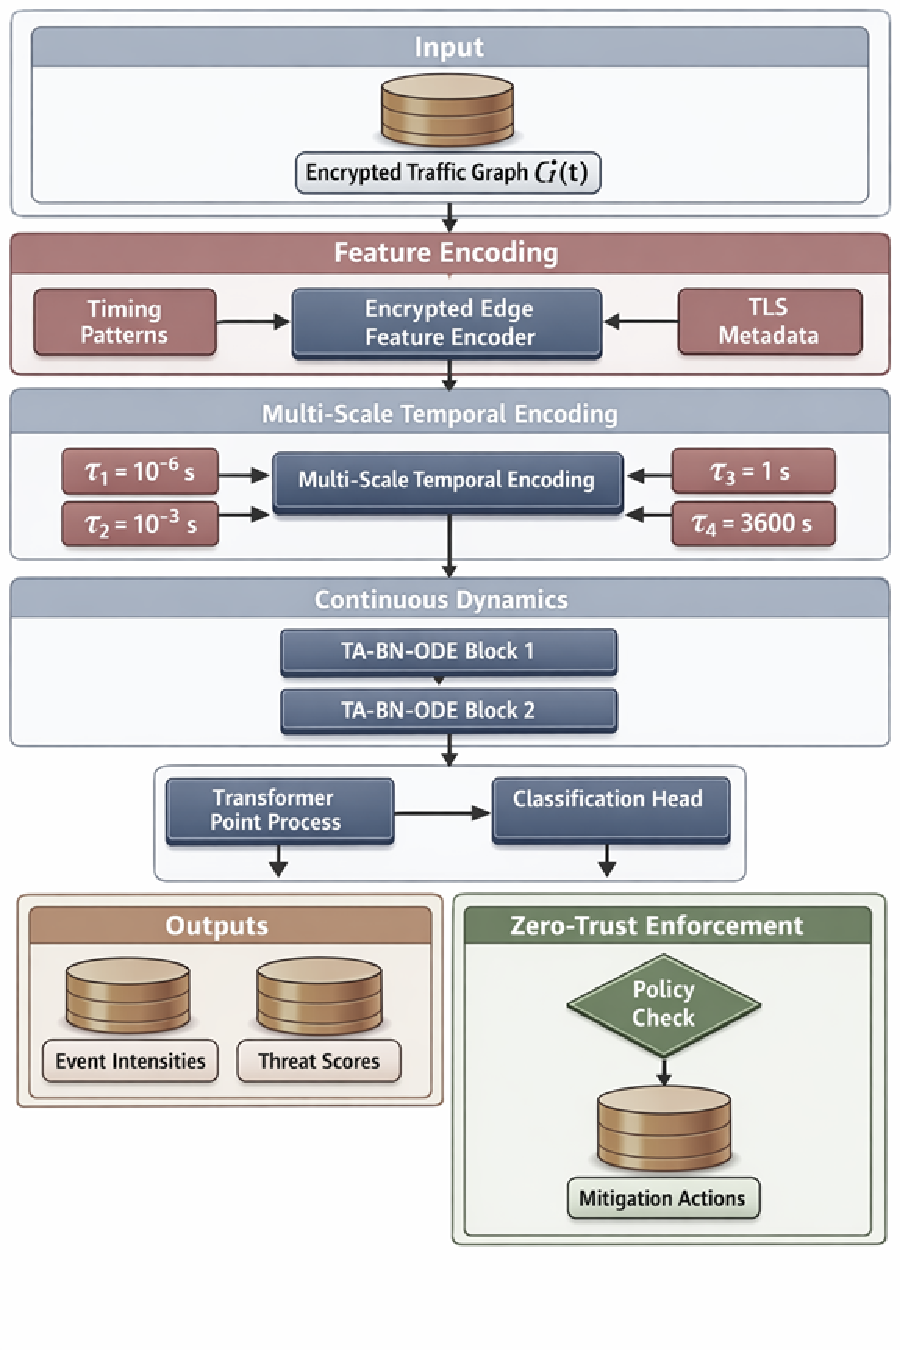
\includegraphics[width=0.75\textwidth]{figures/fig_CT-TGNN_architecture.pdf}
\caption{Архитектура CT-TGNN, реализованная для динамики сетевого трафика.}
\label{fig:ct_tgnn_arch}
\end{figure}

\subsection{М2: FedLLM-API для совместной разведки угроз}

FedLLM-API~\cite{Anaedevha2026neurips} реализован для совместной разведки угроз. Каждый федеративный клиент соответствует центру операций безопасности, владеющему локальными наборами данных трафика. Византийско-устойчивая агрегация (Алгоритм~\ref{alg:fedllm}) защищает от скомпрометированных участников, отправляющих отравленные обновления градиентов. Дифференциальная приватность через локальную обрезку градиентов при пороге $C=1.0$ и гауссовский шум с масштабом $\sigma=0.8$ обеспечивает гарантию $(\epsilon{=}0.85,\delta{=}10^{-5})$ за 100 раундов коммуникации. Выравнивание ОТ Синкхорна с регуляризацией $\lambda=0.1$ корректирует распределительную гетерогенность между центрами. Вес ансамбля LLM $\lambda_{\mathrm{LLM}}=0.3$.

\begin{figure}[htbp]
\centering
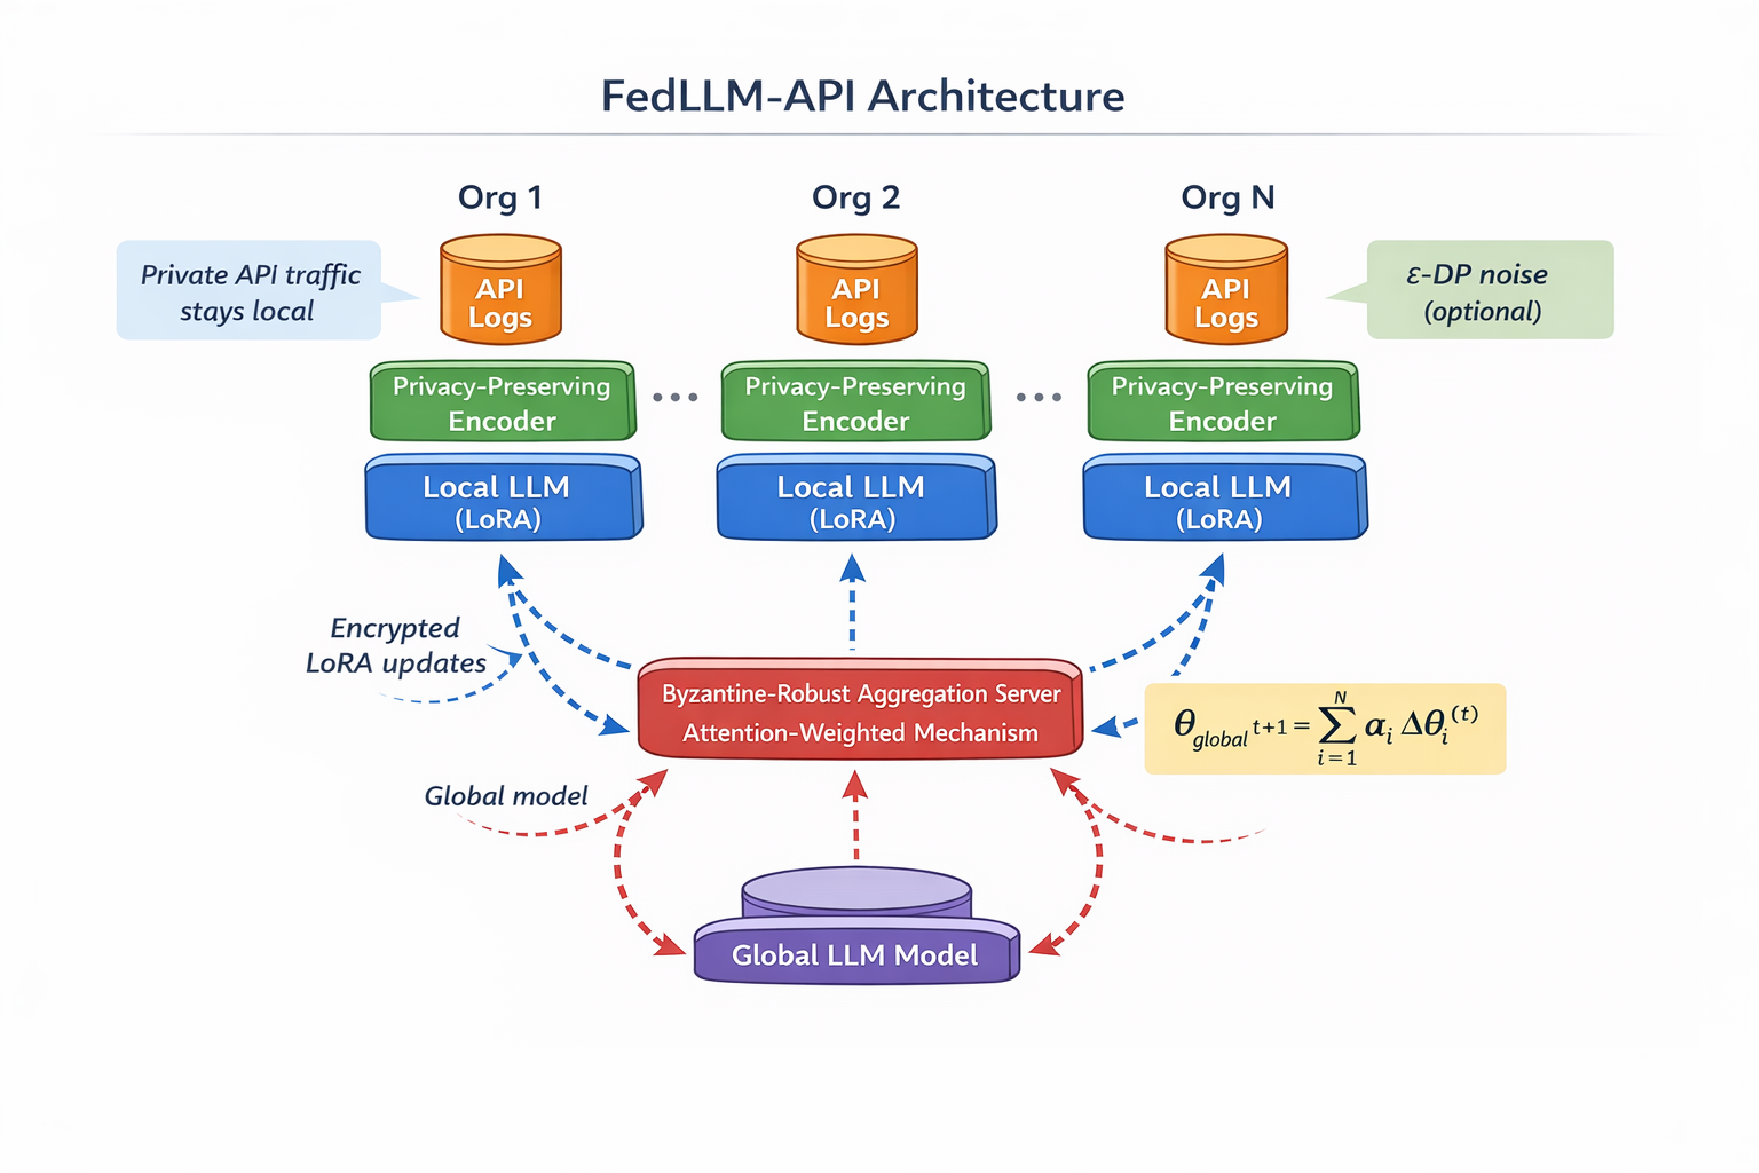
\includegraphics[width=0.78\textwidth]{figures/fig_fedllm_api_architecture.pdf}
\caption{Архитектура FedLLM-API для совместной разведки угроз через организационные границы.}
\label{fig:fedllm_arch}
\end{figure}

\subsection{М3: TripleE-TGNN для многоуровневого мониторинга безопасности}

Граф сервисов $\calG_s(t)$ имеет узлы, представляющие микросервисы, и рёбра, представляющие API-вызовы. Граф трассировок $\calG_r(t)$ имеет узлы, представляющие распределённые трассировки. Граф хостов $\calG_n(t)$ имеет узлы, представляющие узлы инфраструктуры. Сила консолидации EWC $\lambda_{\mathrm{ewc}}=0.5$ балансирует пластичность и стабильность при эволюции топологии. Веса многозадачных потерь $\lambda_s=0.4$, $\lambda_r=0.3$, $\lambda_n=0.3$ с весом согласованности $\lambda_{\mathrm{con}}=0.1$.

\begin{figure}[htbp]
\centering
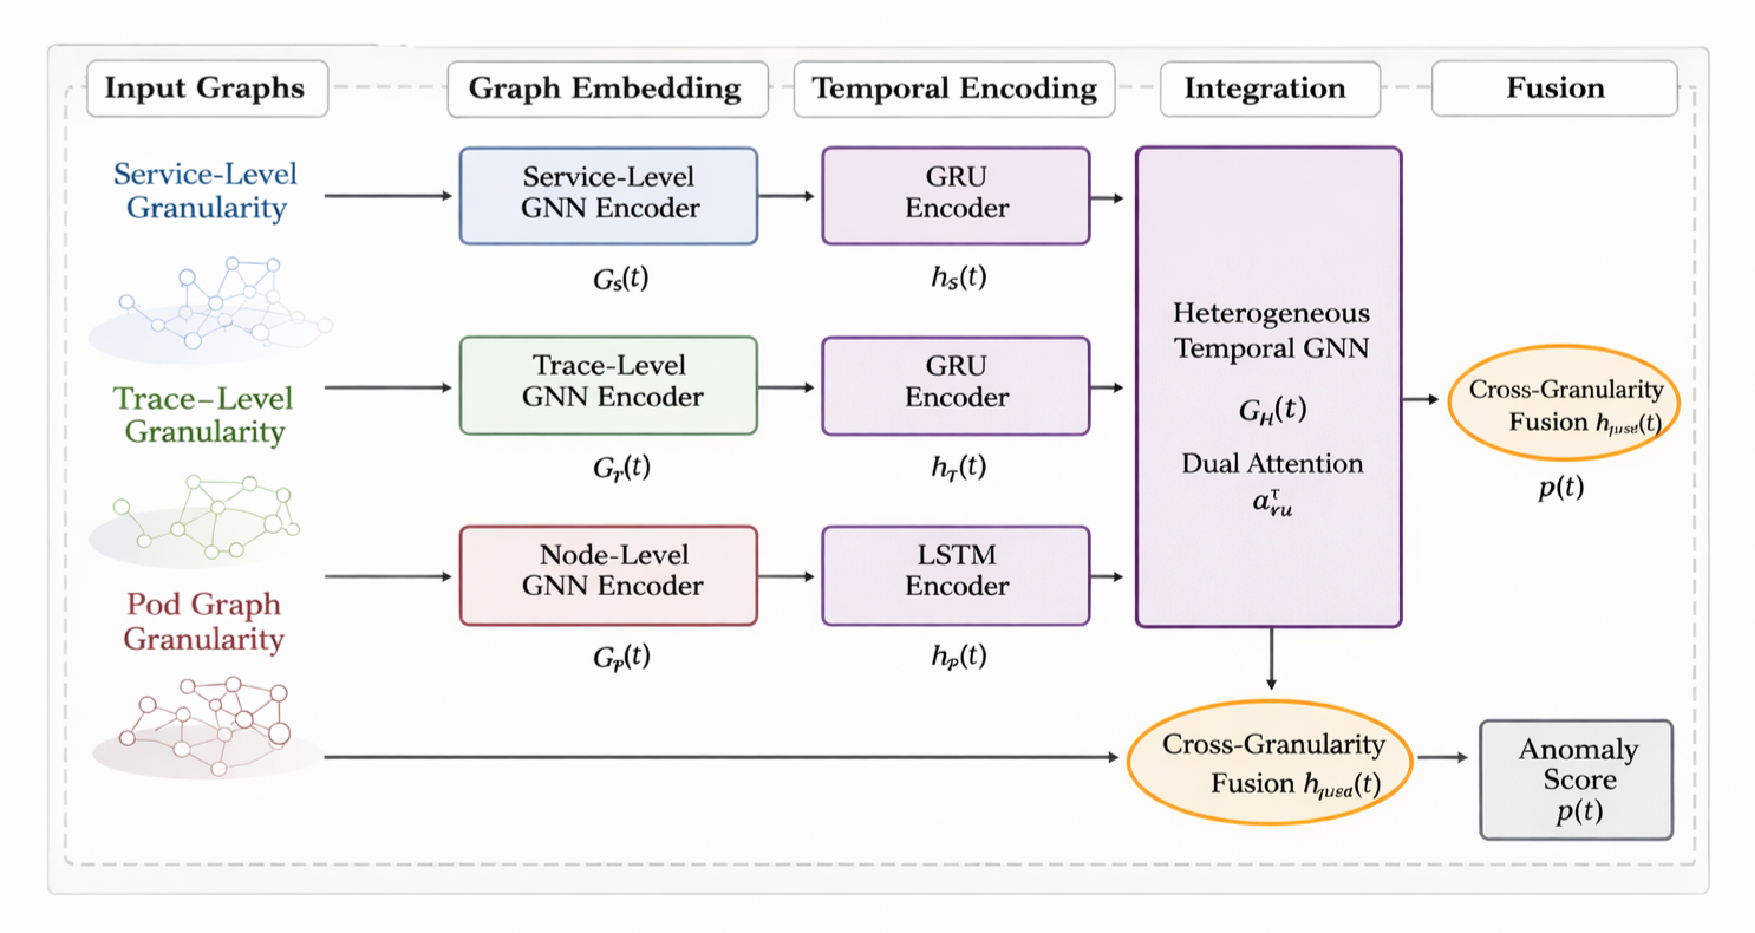
\includegraphics[width=0.82\textwidth]{figures/fig_triplee_tgnn_architecture.pdf}
\caption{Архитектура TripleE-TGNN для многоуровневого мониторинга безопасности в облачных средах.}
\label{fig:triplee_arch}
\end{figure}

\subsection{М4: MambaShield для обнаружения с адаптацией к дрейфу}

MambaShield~\cite{Anaedevha2026mamba} реализован для обнаружения с адаптацией к дрейфу. Последовательные записи потоков обрабатываются селективной моделью пространства состояний, входозависимые переходы которой адаптируются к текущему режиму трафика. Размерность состояния $d_s=64$, шаг дискретизации $\Delta=0.01$ и длина свёрточного ядра БПФ $L=1024$. Ансамбль учителей включает $M=5$ моделей, обученных на непересекающихся подмножествах данных. Учебный план начинается с доли отравления $\rho_0=0.05$ и увеличивается до $\rho_{\max}=0.3$. Дисперсия априорного PAC-Байеса $\sigma_P^2=1.0$.

\begin{figure}[htbp]
\centering
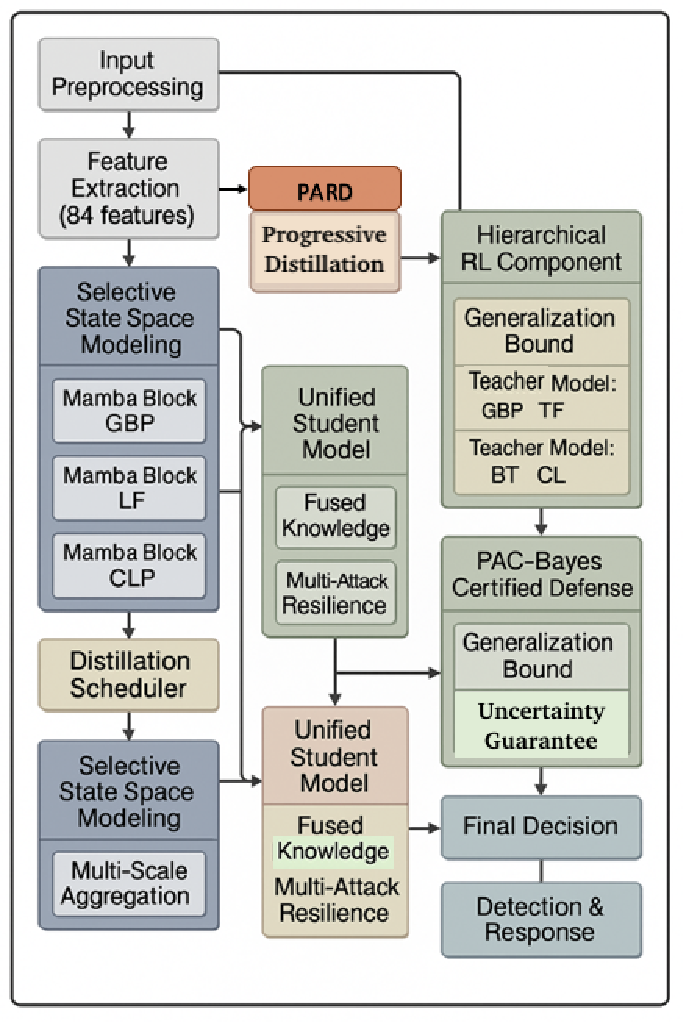
\includegraphics[width=0.75\textwidth]{figures/fig_mambashield_architecture.pdf}
\caption{Архитектура MambaShield для обнаружения вторжений с адаптацией к дрейфу и прогрессивной дистилляцией робастности.}
\label{fig:mamba_arch}
\end{figure}

\subsection{М5/М6: Оценка угроз с калиброванной неопределённостью}

Стохастический трансформер использует $M=50$ прямых проходов Монте-Карло при выводе для получения оценок эпистемической и алеаторной неопределённости. Предсказания с эпистемической неопределённостью, превышающей порог $\tau=0.3$, направляются аналитикам, снижая утомление от оповещений на 43\%. Модуль UC-HGP обеспечивает неопределённость на иерархических гауссовских процессах на временных масштабах, соответствующих ветвям CT-TGNN ($\tau_1$, $\tau_2$, $\tau_3$). Скорость вариационного обучения $\alpha_\phi=5\times10^{-4}$; скорость обучения возмущений $\alpha_\psi=10^{-3}$.

\begin{figure}[htbp]
\centering
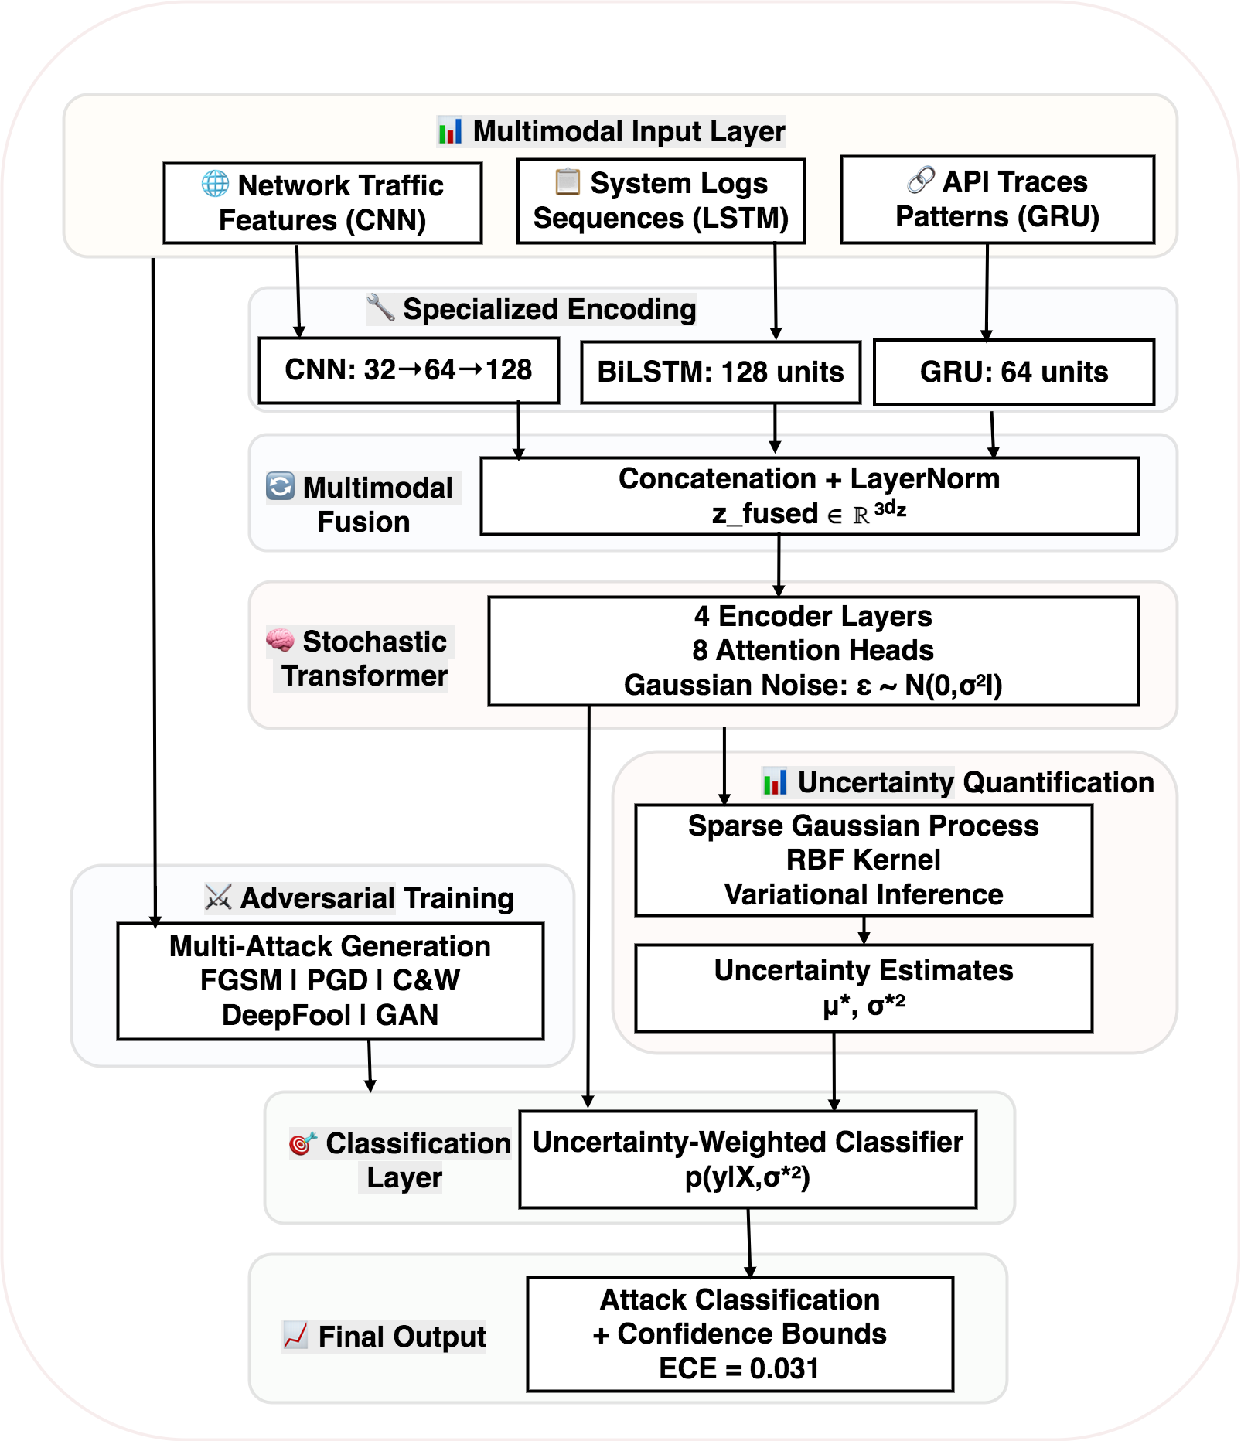
\includegraphics[width=0.82\textwidth]{figures/fig_stochastic_transformer_architecture.pdf}
\caption{Стохастический трансформер с сортировкой на основе неопределённости для операций безопасности.}
\label{fig:stochastic_arch}
\end{figure}

\subsection{М7: Теоретико-игровая система для адаптивных противников}

Пространство действий защитника $\calC$ включает конфигурации обнаружения: покрытие мониторинга, пороги оповещений и политики реагирования. Пространство действий противника $\calA$ охватывает выбор цели, тип возмущения и стратегию уклонения. Скорость обучения мультипликативных весов $\eta=\sqrt{\log|\calC|/T}$. Штраф за неопределённость $\kappa=0.5$; порог направления эксперту $\tau=0.3$.

\begin{figure}[htbp]
\centering
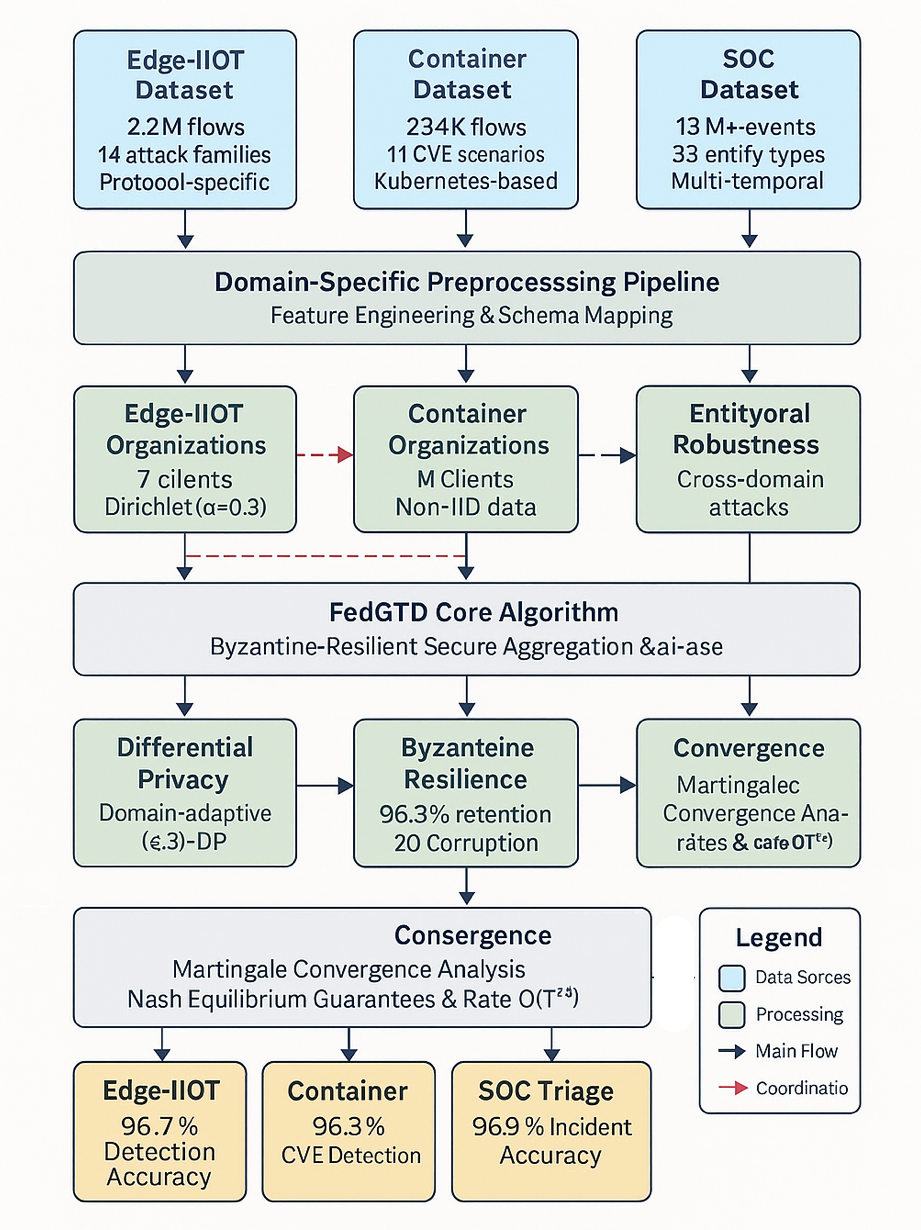
\includegraphics[width=0.86\textwidth]{figures/fig_game_theoretical_architecture.pdf}
\caption{Теоретико-игровая система для адаптивных графовых противников в сетевой безопасности.}
\label{fig:game_arch}
\end{figure}

\subsection{Прямо совместимое обнаружение для постквантовых протоколов}

Протокол-специфичные кодировщики~\cite{Anaedevha2026edm,NIST2024,Regev2009} обрабатывают признаки тайминга для протоколов на основе решёток (Kyber/Dilithium~\cite{Avanzi2022}), структурные признаки для протоколов на основе кодов (McEliece/Niederreiter) и хэш-признаки (SPHINCS+). Слияние кросс-вниманием объединяет три представления. Бюджет состязательного обучения $\epsilon=0.03$ с возмущениями PGD-40.

\begin{figure}[htbp]
\centering
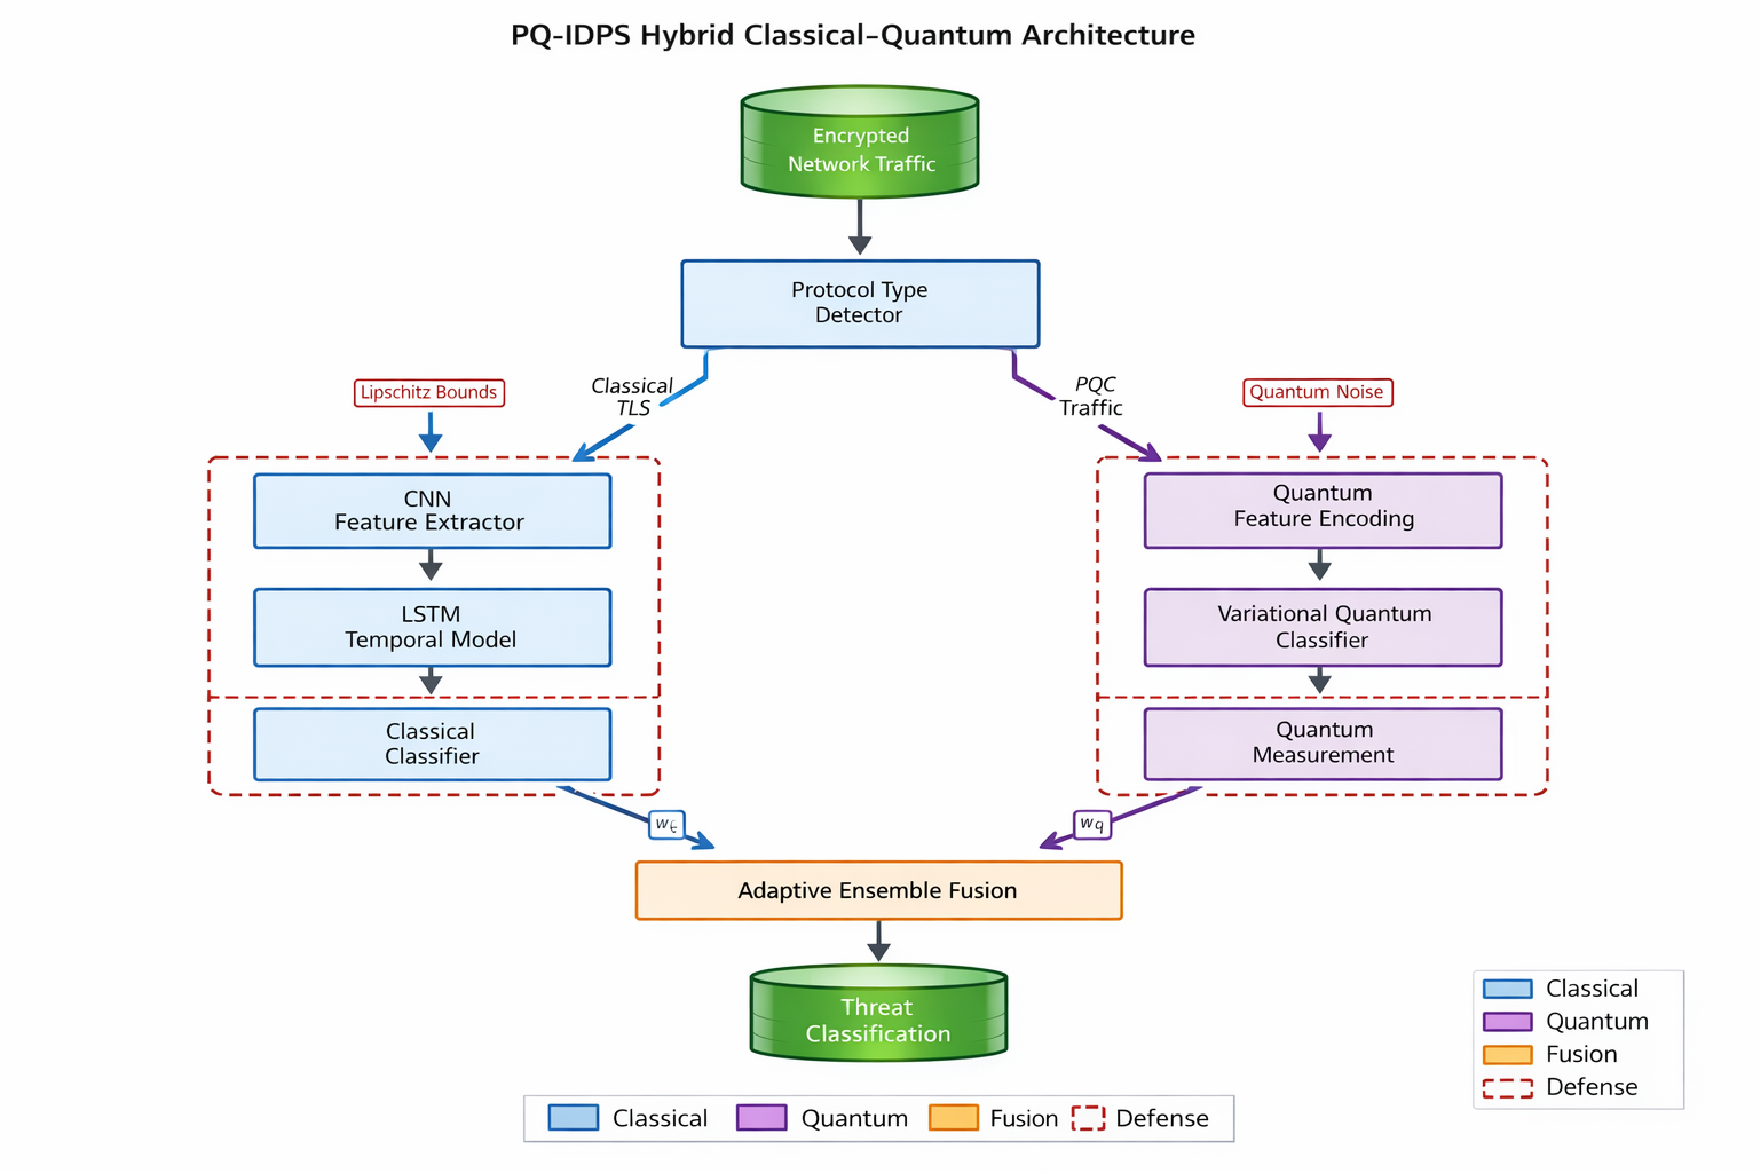
\includegraphics[width=0.82\textwidth]{figures/fig_pq_idps_architecture.pdf}
\caption{Прямо совместимая мультипротокольная архитектура обнаружения для постквантового трафика.}
\label{fig:pqidps_arch}
\end{figure}

%%=====================================================================
\section{Инфраструктура развёртывания и интеграции системы}
\label{sec:tech_stack_ui}
%%====

\subsection{Технологический стек реализации}
\label{subsec:tech_stack}

Программная платформа RobustIDPS.ai представляет собой
\emph{единое веб-приложение прогрессивного типа}
(Progressive Web Application, PWA) с разделением на серверный и
клиентский ярусы, контейнеризованное средствами Docker~Compose и
оркестрируемое единым backend-/инференс-процессом. Стек технологий
выбран таким образом, чтобы обеспечить одновременно: (i)~воспроизводимое
обучение и инференс глубоких графовых нейросетевых моделей М1--М7;
(ii)~устойчивую потоковую обработку сетевого трафика в режиме
реального времени; (iii)~интерактивный пользовательский интерфейс
аналитика SOC; (iv)~интеграцию с внешними поставщиками больших
языковых моделей (LLM) через единый API-абстрактный слой.

\begin{enumerate}[leftmargin=2em, itemsep=0pt]
\item \textbf{Серверный ярус (Python~3.11)}~--- асинхронный
HTTP/WebSocket-сервер на FastAPI (60+ конечных точек REST API),
поверх которого исполняется модельный конвейер на PyTorch~2.x с
расширениями PyTorch~Geometric и DGL для графовых операций;
обработка пакетного трафика опирается на NFStream для
извлечения flow-признаков из PCAP и на dpkt/Scapy для разбора
сырого трафика; служебные очереди и Pub/Sub реализованы на
Redis~7 (cache + queue), персистентное хранение бенчмарков и
журналов инцидентов~--- PostgreSQL~16.

\item \textbf{Клиентский ярус (TypeScript / React~18)}~---
прогрессивное веб-приложение из \textbf{51~страницы}
пользовательского интерфейса, объединённых в десять
функциональных групп (см.~подраздел~\ref{subsec:ui_walkthrough}).
Real-time-обновления потоковой классификации передаются по
WebSocket; визуализация графов и метрик~--- Recharts и собственная
графовая визуализация на D3.js; стилизация~--- Tailwind~CSS с
тёмной темой по умолчанию.

\item \textbf{Ярус интеграции LLM}~--- единый абстрактный
интерфейс LLM-провайдера с реализациями для четырёх
коммерческих бэкендов (Anthropic Claude, OpenAI GPT-4o,
Google Gemini, DeepSeek) и для локального инференса;
четырёхуровневая система защиты LLM (Prompt Injection,
Jailbreak, RAG~Poisoning, Multi-Agent Chain) реализована как
прозрачный middleware-слой между UI и провайдерами.

\item \textbf{Ярус развёртывания}~--- контейнеризация Docker
с многоэтапной сборкой и Compose-оркестрацией; интеграция с
существующими средствами защиты информации обеспечена
плагином для EVE-JSON формата Suricata, что позволяет
встраивать RobustIDPS.ai в действующую СОВ организации без
изменения существующих сигнатурных правил (что подтверждается
актом внедрения ООО <<НИИ~ИКТ>>, см.~Главу~\ref{ch:platform}).

\end{enumerate}

\subsection{Используемые пакеты и версии}
\label{subsec:packages_versions}

В таблице~\ref{tab:packages_versions} приведены ключевые
программные зависимости платформы RobustIDPS.ai с указанием
версий, использованных при подготовке экспериментальных
результатов и при подписании актов внедрения. Полный
\texttt{requirements.txt} и \texttt{package.json} депонированы
вместе с исходным кодом на Zenodo (DOI:~10.5281/zenodo.19129512).

\begin{table}[H]
\centering
\caption{Программные зависимости платформы RobustIDPS.ai}
\label{tab:packages_versions}
\small
\renewcommand{\arraystretch}{0.92}\begin{tabular}{@{}lll@{}}
\toprule
\textbf{Категория} & \textbf{Пакет} & \textbf{Версия} \\
\midrule
Язык реализации & Python & 3.11.x \\
Веб-сервер & FastAPI & 0.110+ \\
ASGI-сервер & Uvicorn (uvloop) & 0.27+ \\
Глубокое обучение & PyTorch & 2.2+ \\
Графовые операции & PyTorch~Geometric & 2.5+ \\
Графовые операции (доп.) & DGL & 2.1+ \\
Нейронные ОДУ & torchdiffeq & 0.2.4 \\
Модели пространства состояний & mamba-ssm & 1.2+ \\
Извлечение flow-признаков & NFStream & 6.5+ \\
Разбор сырых пакетов & dpkt~/~Scapy & 1.9~/~2.5 \\
Хранилище & PostgreSQL & 16 \\
Кэш и очереди & Redis & 7 \\
Контейнеризация & Docker & 24+ \\
Оркестрация & Docker Compose & v2 \\
Клиент (язык) & TypeScript & 5.3+ \\
Клиент (фреймворк) & React & 18 \\
Сборка клиента & Vite & 5 \\
UI-библиотека & Tailwind CSS & 3.4 \\
Визуализация графиков & Recharts & 2.10 \\
Визуализация графов & D3.js & 7 \\
Real-time-обновления & WebSocket (стандарт RFC~6455) & --- \\
LLM-провайдеры (API) & anthropic, openai, google-genai, deepseek & акт. \\
Сигнатурный плагин & Suricata EVE-JSON & 7.0 (совместимость) \\
\bottomrule
\end{tabular}
\end{table}

\subsection{Пользовательский интерфейс и демонстрация
практического применения}
\label{subsec:ui_walkthrough}

Пользовательский интерфейс RobustIDPS.ai разработан как
\emph{единая точка входа} для всех ролей кибербезопасности
организации: оператор SOC, аналитик по реагированию на
инциденты, инженер ML-моделей, аудитор соответствия. Интерфейс
объединяет 51~страницу, сгруппированных в десять функциональных
групп: <<AI Command Centre>>, <<AI Data \& Models>>, <<AI Active
Defence>>, <<SOC Intelligence>>, <<AI Novel Methods>>,
<<LLM Attack Surfaces>>, <<MLSecOps Standards>>,
<<AI Security \& Gov>>, <<Industry \& Research>> и
<<Notice Board>>. Ниже на рис.~\ref{fig:gui_walkthrough_p1}
приведена демонстрация практической работы платформы в порядке
типичного сценария использования аналитиком.

\begin{figure}[htbp]
\centering
\setlength{\fboxsep}{0pt}\setlength{\fboxrule}{0.4pt}
\renewcommand{\arraystretch}{0.92}\begin{tabular}{@{}c@{\hspace{4pt}}c@{\hspace{4pt}}c@{}}
\fbox{
\includegraphics[width=0.31\textwidth,height=2.6cm,keepaspectratio]{figures/gui/gui_01_login.png}} &
\fbox{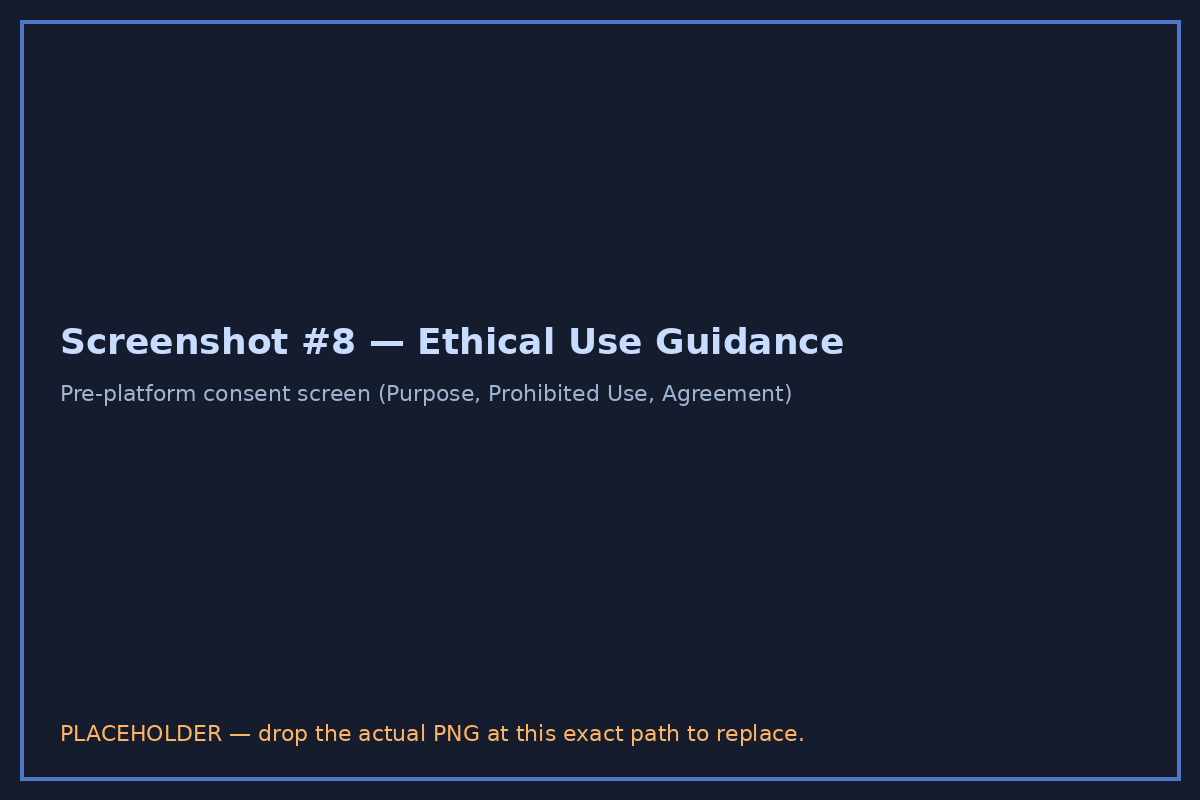
\includegraphics[width=0.31\textwidth,height=2.6cm,keepaspectratio]{figures/gui/gui_08_ethical_use.png}} &
\fbox{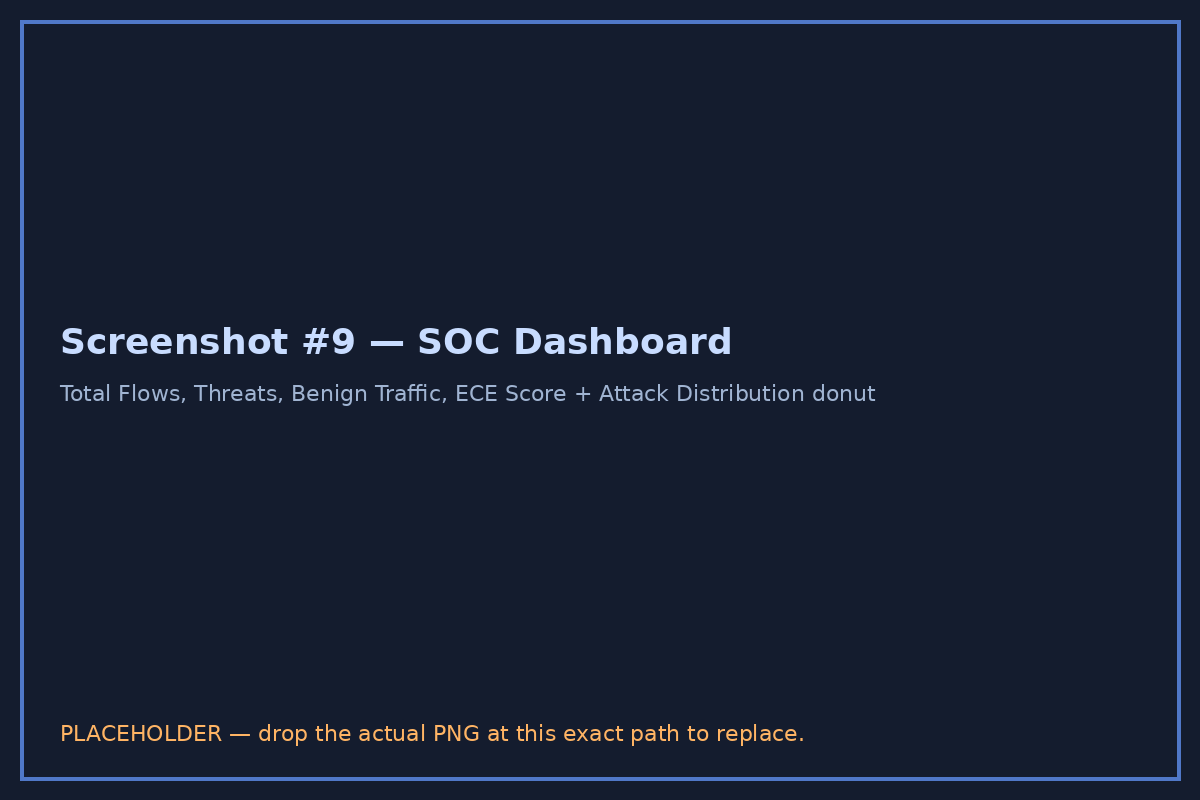
\includegraphics[width=0.31\textwidth,height=2.6cm,keepaspectratio]{figures/gui/gui_09_soc_dashboard.png}} \\
\scriptsize (а) Аутентификация &
\scriptsize (б) Этические требования и согласие &
\scriptsize (в) Панель SOC \\[4pt]
\fbox{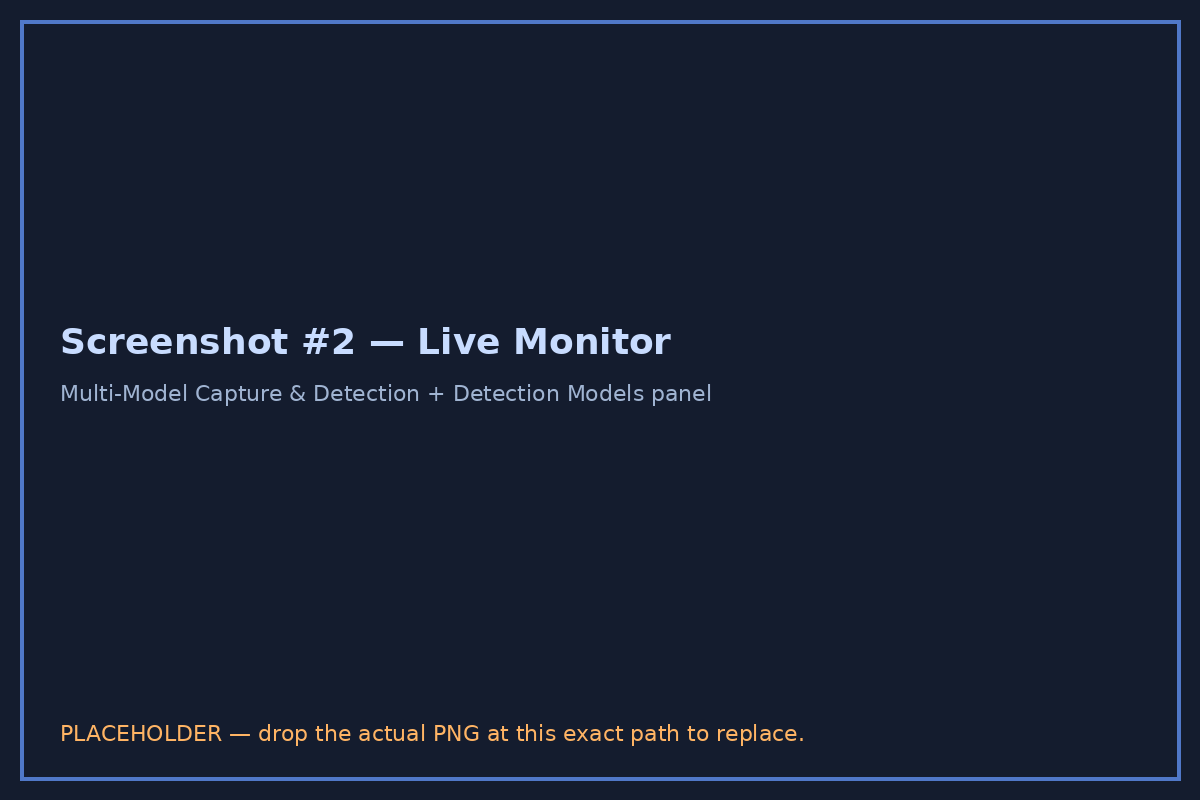
\includegraphics[width=0.31\textwidth,height=2.6cm,keepaspectratio]{figures/gui/gui_02_live_monitor.png}} &
\fbox{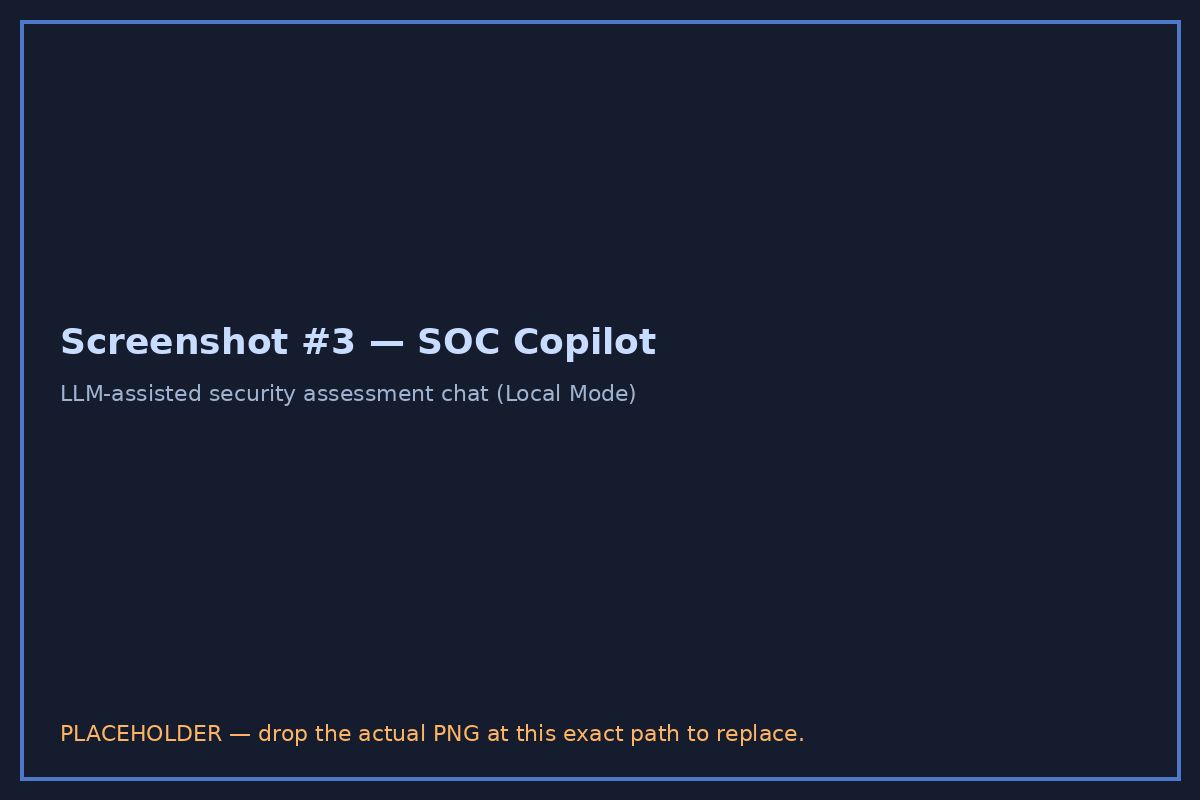
\includegraphics[width=0.31\textwidth,height=2.6cm,keepaspectratio]{figures/gui/gui_03_soc_copilot.png}} &
\fbox{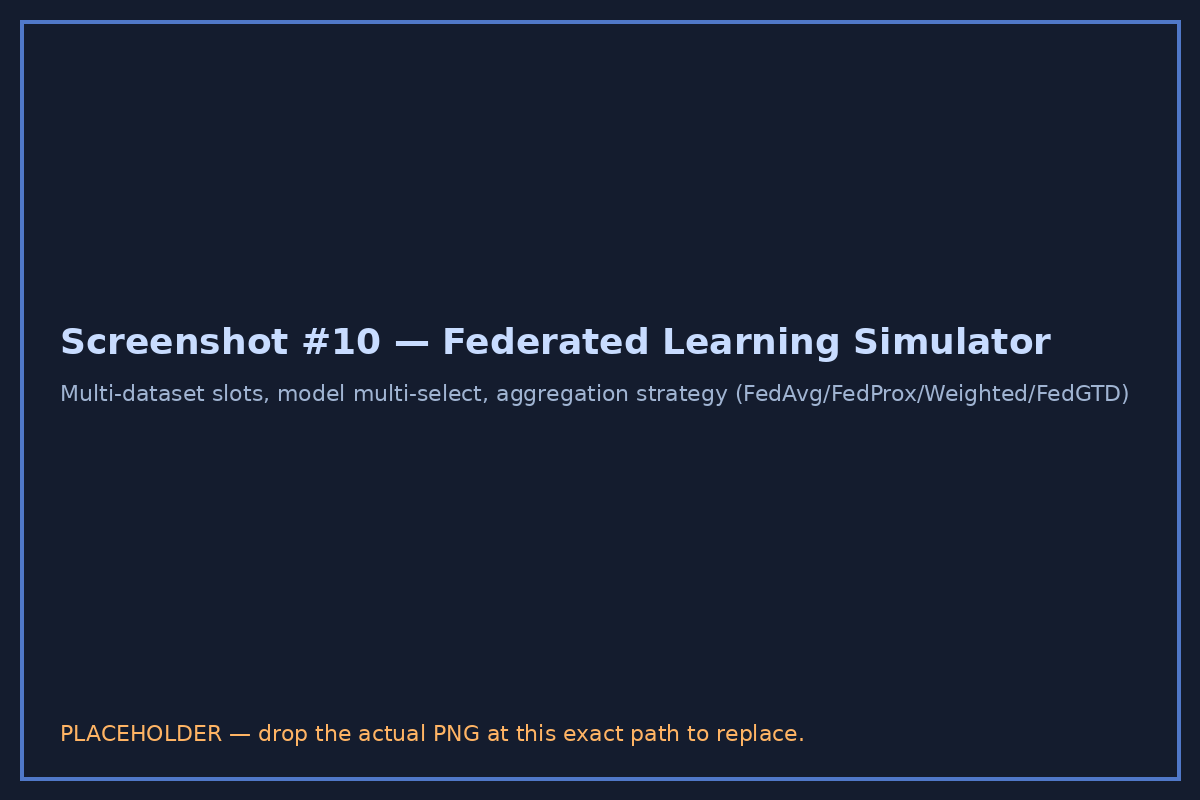
\includegraphics[width=0.31\textwidth,height=2.6cm,keepaspectratio]{figures/gui/gui_10_fed_learning.png}} \\
\scriptsize (г) Live Monitor &
\scriptsize (д) SOC Copilot (LLM-ассистент) &
\scriptsize (е) Симулятор федеративного обучения \\
\end{tabular}
\caption{Демонстрация практической работы RobustIDPS.ai
(часть~1)~--- от входа в систему до распределённого обучения:
\textbf{(а)}~страница входа с аутентификацией по электронной
почте и паролю и регистрацией нового пользователя;
\textbf{(б)}~страница <<Этические требования и согласие>>~---
обязательное подтверждение допустимых сценариев использования
(академические исследования, авторизованное тестирование на
проникновение, государственные и оборонные исследования,
оценочные исследования) и запрещённых действий, реализующее
требование MLSecOps к процедуре допуска оператора;
\textbf{(в)}~страница SOC Dashboard~--- сводка по 1\,000 потокам,
347 обнаруженным угрозам, 65{,}3\,\% доли доброкачественного
трафика и текущей оценке калибровки ECE\,=\,0{,}043 с
распределением по пяти уровням серьёзности и каноническим
диаграммам распределения атак и доверия;
\textbf{(г)}~страница Live Monitor~--- запуск потокового
захвата сетевого интерфейса \texttt{eth0} с выбором ансамбля из
семи моделей обнаружения (SurrogateIDS, Neural~ODE,
Optimal~Transport, FedGTD, SDE-TGNN, CyberSecLLM и др.) и
регулировкой интервала захвата 5--120~с;
\textbf{(д)}~страница SOC Copilot~--- интерактивный
LLM-ассистент в локальном режиме, отвечающий на запрос
аналитика <<Получить результаты Live Monitor с разбивкой по
угрозам, серьёзности и доверию>> по реальным данным сессии
захвата;
\textbf{(е)}~страница Federated Learning Simulator~--- запуск
федеративного обучения по нескольким наборам данных
одновременно (CSV/PCAP-слоты Slot\,1--3) с выбором стратегии
агрегации (FedAvg, FedProx, Weighted, FedGTD), режима IID/Non-IID
и опции дифференциальной приватности.}
\label{fig:gui_walkthrough_p1}
\end{figure}

\begin{figure}[htbp]
\centering
\setlength{\fboxsep}{0pt}\setlength{\fboxrule}{0.4pt}
\renewcommand{\arraystretch}{0.92}\begin{tabular}{@{}c@{\hspace{4pt}}c@{\hspace{4pt}}c@{}}
\fbox{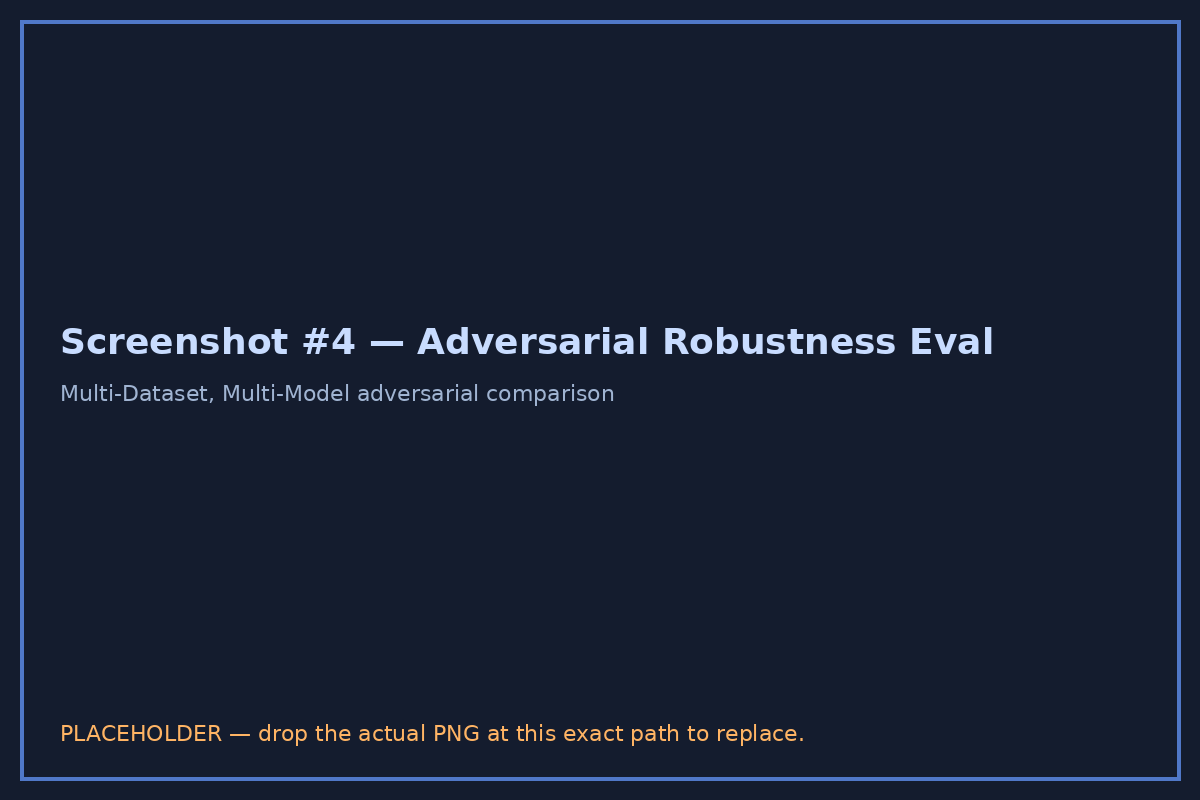
\includegraphics[width=0.31\textwidth,height=2.6cm,keepaspectratio]{figures/gui/gui_04_adversarial_eval.png}} &
\fbox{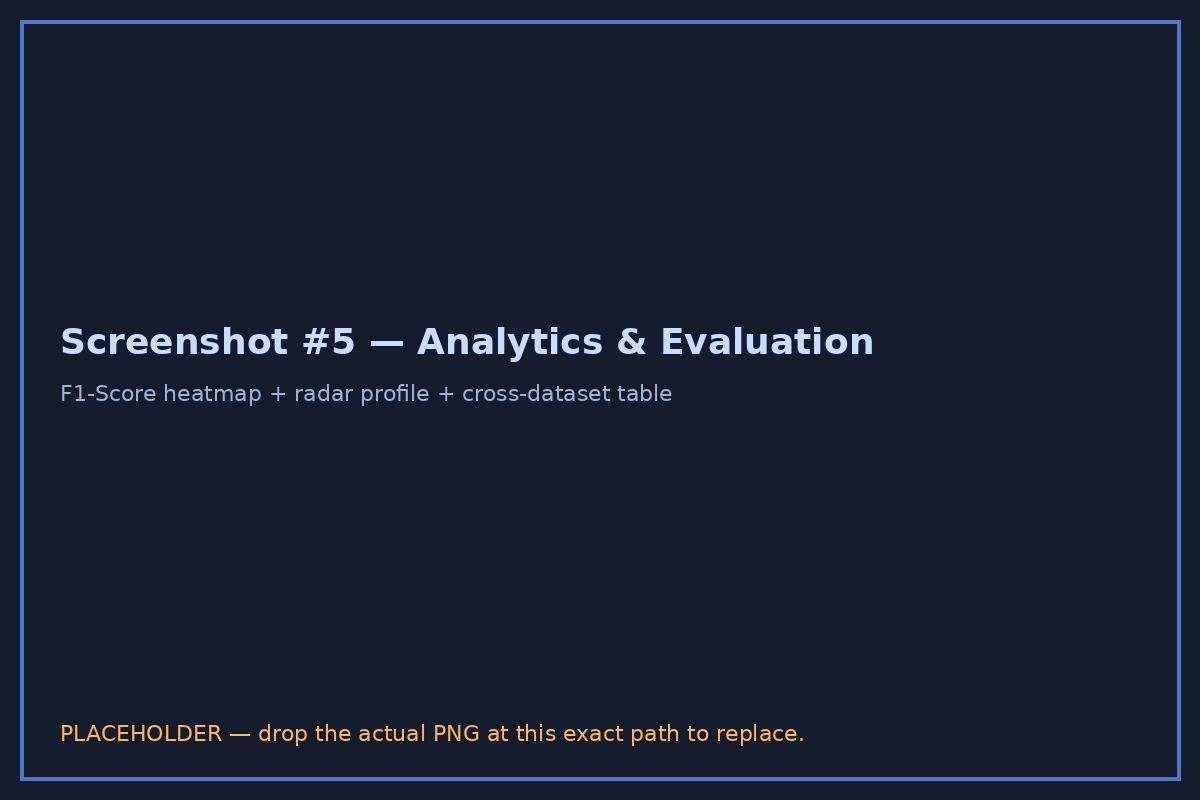
\includegraphics[width=0.31\textwidth,height=2.6cm,keepaspectratio]{figures/gui/gui_05_analytics_charts.png}} &
\fbox{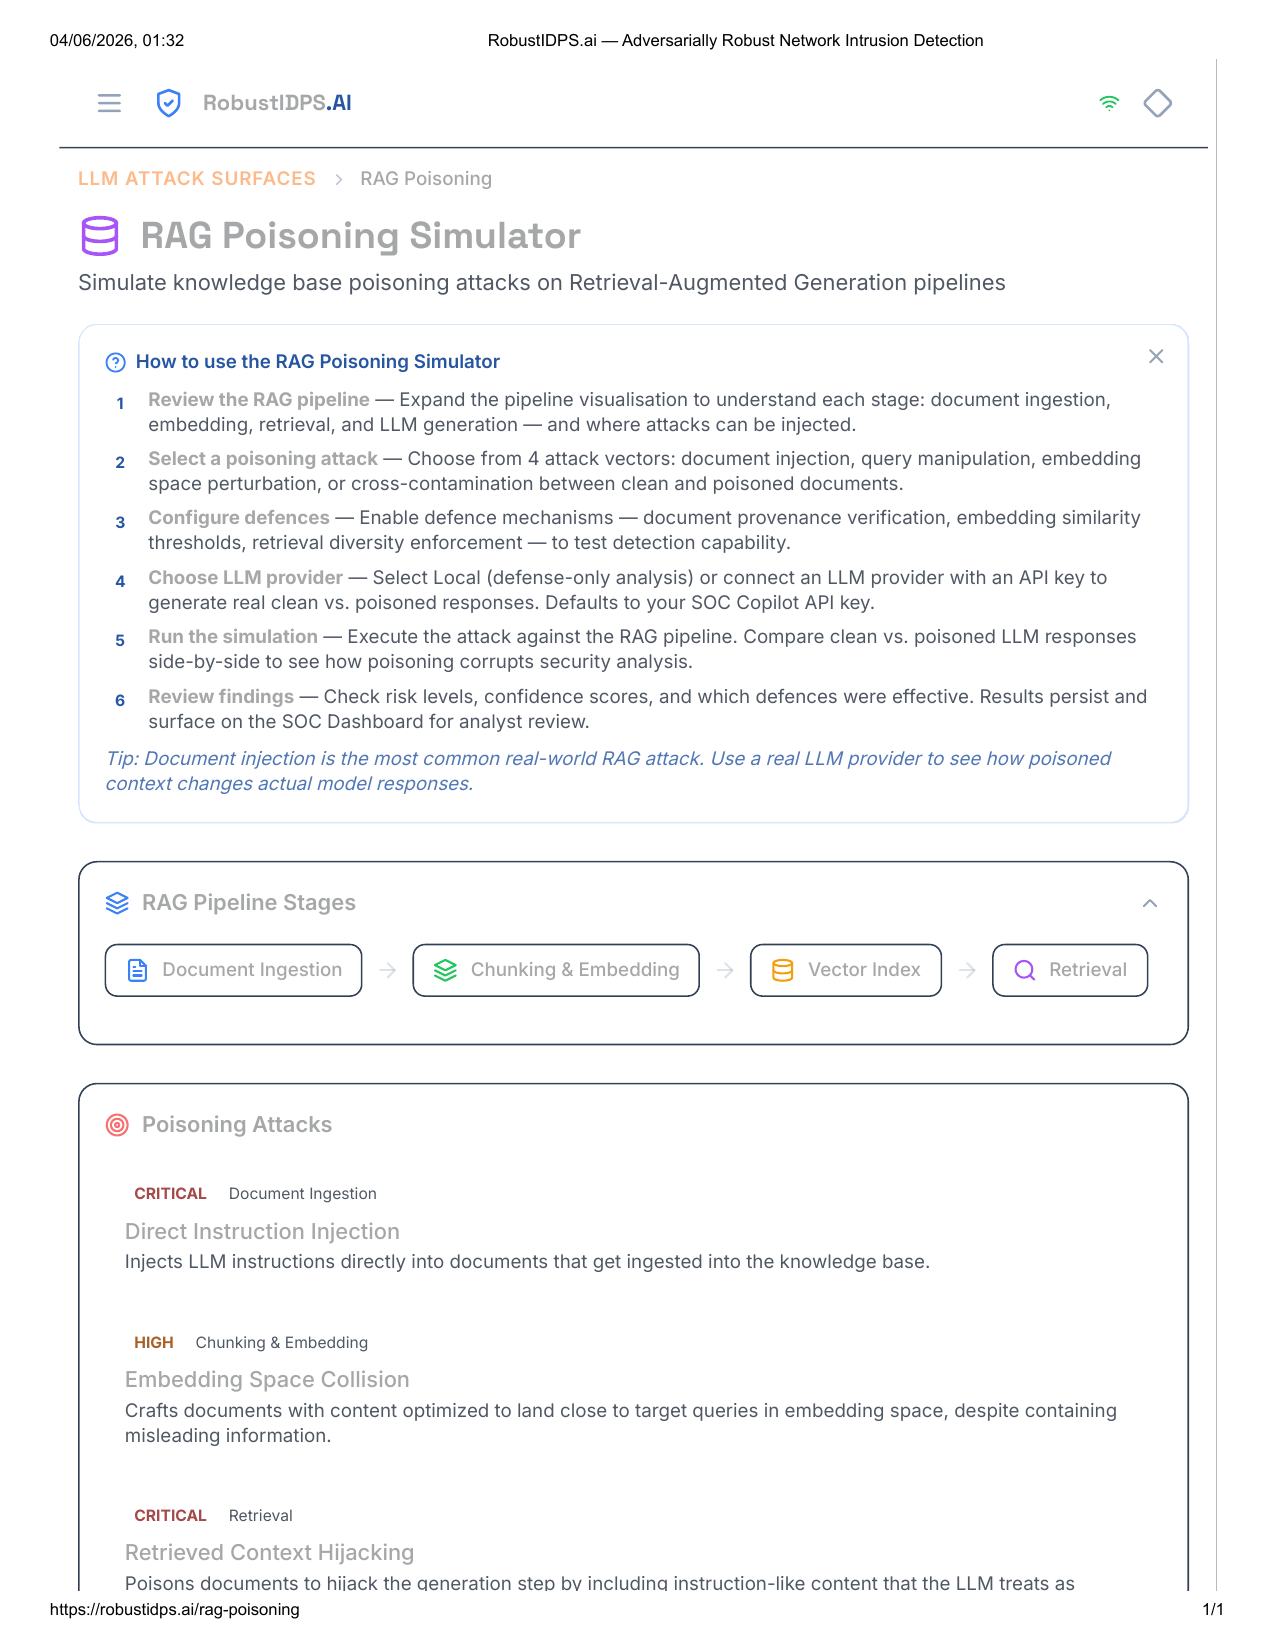
\includegraphics[width=0.31\textwidth,height=2.6cm,keepaspectratio]{figures/gui/gui_07_rag_poisoning.png}} \\
\scriptsize (ж) Сравнение моделей по робастности &
\scriptsize (з) Аналитика и оценка качества &
\scriptsize (и) Симулятор отравления RAG \\
\end{tabular}
\caption{Демонстрация практической работы RobustIDPS.ai
(часть~2)~--- состязательное тестирование, аналитика и атаки на
LLM: \textbf{(ж)}~страница Adversarial~Eval~--- мультидатасетное
сравнение моделей по устойчивости к шести методам состязательных
атак (FGSM, PGD, C\&W, DeepFool, Gaussian noise, Label masking);
\textbf{(з)}~страница Analytics \& Evaluation~--- сравнение
метрик F1 для семи моделей по шести бенчмаркам с тепловой
картой, радар-профилем и таблицей кросс-датасетной
согласованности; \textbf{(и)}~страница RAG Poisoning Simulator~---
симуляция атак на RAG-конвейер LLM с четырьмя векторами атаки
(document injection, query manipulation, embedding space
perturbation, cross-contamination).}
\label{fig:gui_walkthrough_p2}
\end{figure}

\noindent Дополнительный снимок страницы Analytics с открытой
подсказкой <<Как пользоваться>> приведён на
рис.~\ref{fig:gui_analytics_intro}, иллюстрируя пять
встроенных интерактивных пояснений к десяти вкладкам
оценки качества (Performance, Convergence, Robustness, Privacy,
Transfer Learning, Calibration, ROC/AUC, Dataset Comparison,
Statistical Analysis, Cross-Module Intel).

\begin{figure}[htbp]
\centering
\fbox{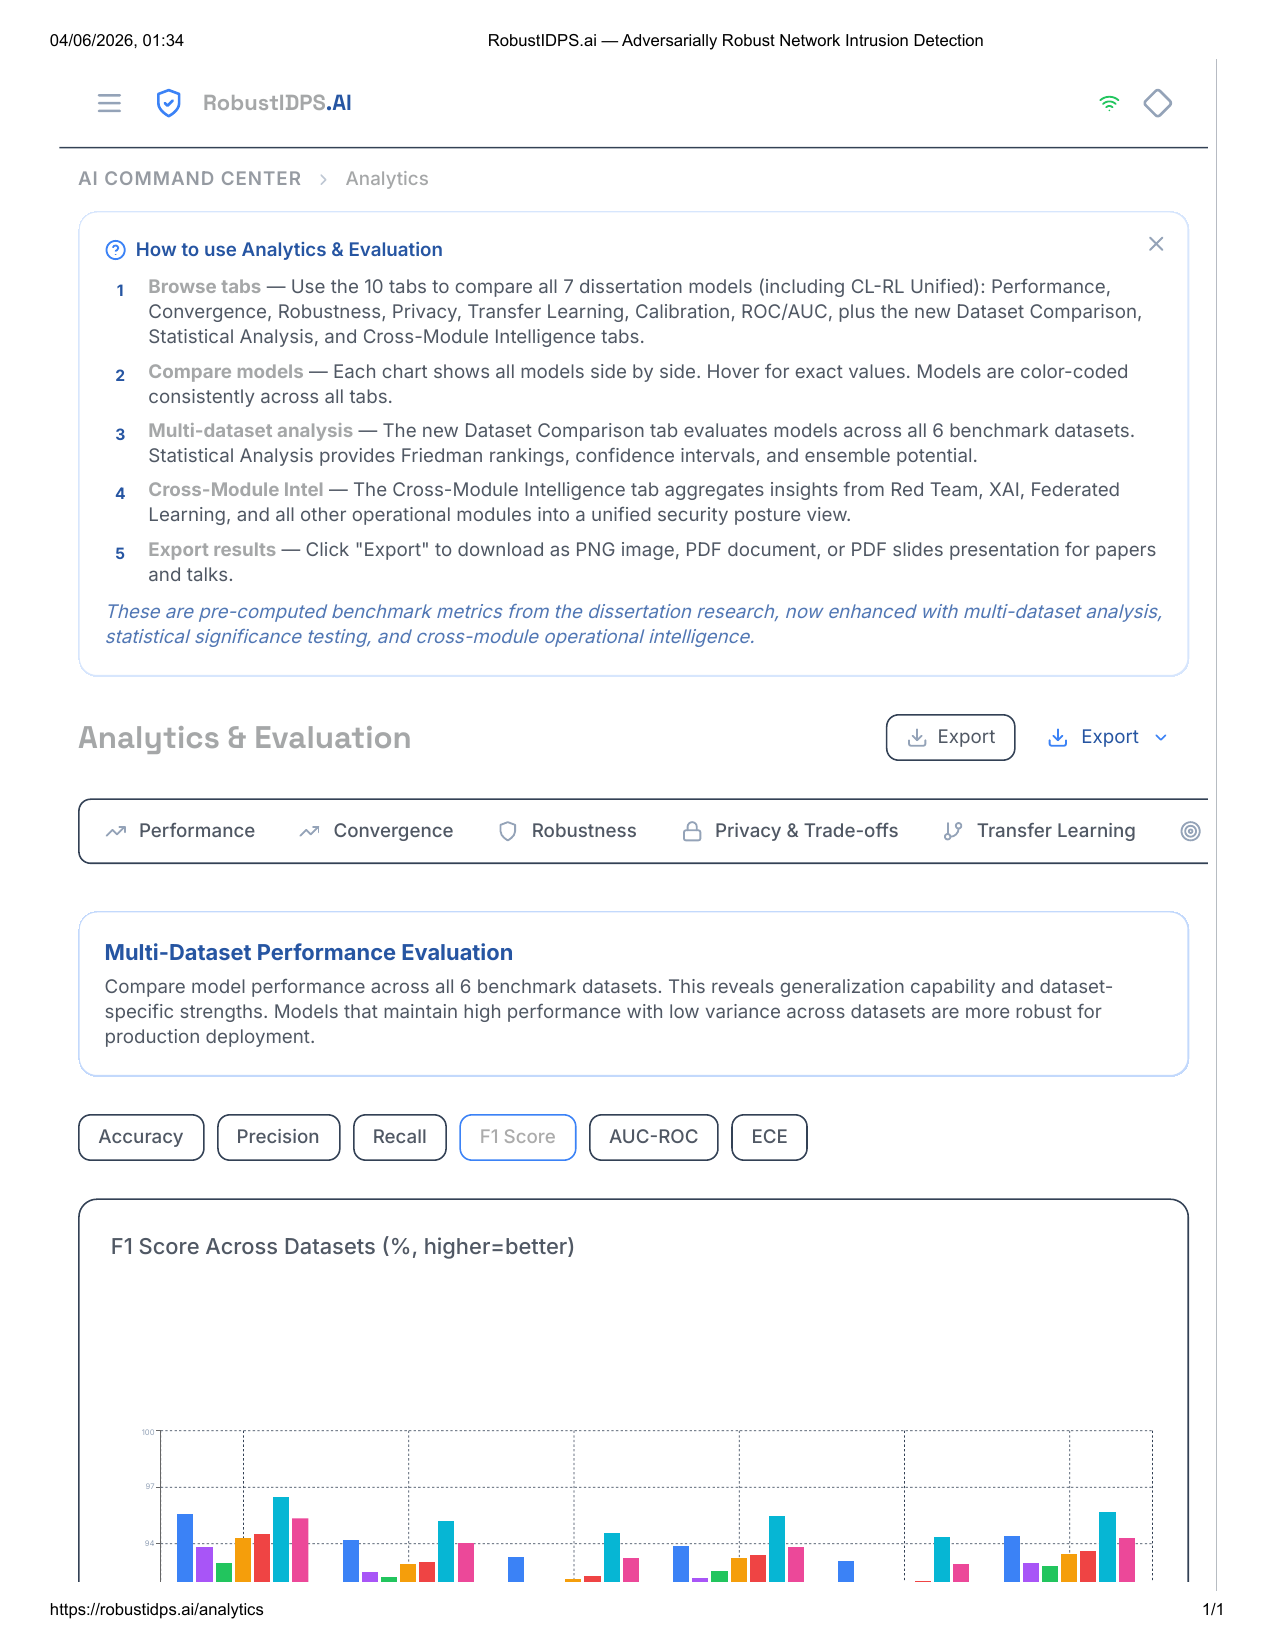
\includegraphics[width=0.86\textwidth]{figures/gui/gui_06_analytics_intro.png}}
\caption{Страница Analytics~\& Evaluation с подсказкой
<<Как пользоваться>>: интерактивные пояснения к десяти вкладкам
сравнительной оценки моделей, экспорт результатов в PNG/PDF и
PDF-презентацию.}
\label{fig:gui_analytics_intro}
\end{figure}

Представленные снимки экрана демонстрируют, что RobustIDPS.ai
реализует все теоретические разработки М1--М7 в виде
\emph{практически развёрнутой} платформы с интерфейсом
промышленного качества; целостность реализации подтверждена
актами внедрения ООО~<<НИИ~ИКТ>> (активное использование
платформы штатными специалистами кибербезопасности) и
ООО~<<Ксайрикс>> (интеграция в действующую систему анализа
сетевого трафика и защиты сетевой инфраструктуры).

%%=====================================================================
\section{Оптимизация производительности системы}
\label{sec:hyperparams}
%%====

Таблица~\ref{tab:hyperparams} объединяет основные гиперпараметры всех методов в конфигурации для области сетевой безопасности. Все значения подобраны поиском по сетке на валидационном наборе CIC-IoT-2023 и подтверждены стабильными на оставшихся пяти наборах данных.

\begin{table}[htbp]\centering\small
\caption{Сводная конфигурация гиперпараметров всех методов для области кибербезопасности.}
\label{tab:hyperparams}
\small
\renewcommand{\arraystretch}{0.92}\begin{tabular}{p{3.5cm} p{2.5cm} p{2.5cm} p{5.0cm}}
\toprule
\textbf{Метод} & \textbf{Параметр} & \textbf{Значение} & \textbf{Обоснование} \\
\midrule
\multirow{4}{3.5cm}{М1: CT-TGNN}
& Скрыт. разм. & 256 & Ёмкость для 83-призн. входа \\
& Допуск ОДУ & $10^{-5}$ & Баланс точности/скорости \\
& Пост. времени & 1/60/3600\,с & Масшт. пакет/сессия/кампания \\
& Граница Липш. & Спектр. норма & Сертифиц. робастность \\
\addlinespace
\multirow{4}{3.5cm}{М2: FedLLM-API}
& Обрезка $C$ & 1.0 & Граница чувствит. ДП \\
& ДП $(\epsilon,\delta)$ & $(0.85, 10^{-5})$ & Строгая гарантия приватн. \\
& Рег. ОТ $\lambda$ & 0.1 & Сходимость Синкхорна \\
& Вес LLM & 0.3 & Баланс ансамбля \\
\addlinespace
\multirow{3}{3.5cm}{М3: TripleE-TGNN}
& EWC $\lambda$ & 0.5 & Предотвращение забывания \\
& Веса уровней & 0.4/0.3/0.3 & Акцент на сервисах \\
& Согласов. $\lambda_{\mathrm{con}}$ & 0.1 & Межуровн. согласованн. \\
\addlinespace
\multirow{3}{3.5cm}{М4: MambaShield}
& Разм. состояния & 64 & Ёмкость SSM \\
& Длина ядра & 1024 & Охват последовательн. \\
& Расп. отравления & 0.05--0.3 & Прогрессивн. закалка \\
\addlinespace
\multirow{3}{3.5cm}{М5/М6: Стох.\ трансф.}
& Выборки МК & 50 & Качество неопределённости \\
& Порог сортировки & 0.3 & Баланс ЛП/ЛО \\
& Калибровка & Температура & Минимизация ECE \\
\addlinespace
\multirow{2}{3.5cm}{М7: Сертификация}
& MWU $\eta$ & $\sqrt{\log|\calC|/T}$ & Оптимальный регрет \\
& Штраф неопр. $\kappa$ & 0.5 & Чувствит. к риску \\
\bottomrule
\end{tabular}
\end{table}

Все методы реализованы на PyTorch~2.1~\cite{Paszke2019} с CUDA~12.1. Обучение использует AdamW с начальной скоростью обучения $2\times10^{-4}$, затуханием весов $10^{-5}$ и косинусным отжигом. Обучение со смешанной точностью снижает потребление памяти на 40\%. Обрезка градиентов при норме 1.0 предотвращает нестабильность. Ранняя остановка с терпением 10 эпох мониторит потери валидации.

%%=====================================================================
\section{Сравнительный анализ архитектурных и функциональных возможностей системы RobustIDPS.ai и существующих систем обнаружения и предотвращения вторжений}
\label{sec:integrated_arch}
%%====

Семь методов (М1--М7) интегрированы в единый конвейер обнаружения, поток данных которого проходит следующим образом. Сырой сетевой трафик поступает через модуль приёма данных, выполняющий разбор протоколов, извлечение потоков и вычисление 83 признаков. Модуль CT-TGNN строит темпоральный граф и вычисляет вложения узлов непрерывного времени. Модуль TripleE-TGNN поддерживает многоуровневые вложения для иерархических сред. Модуль MambaShield обрабатывает последовательные записи событий для оценки с адаптацией к дрейфу. Модули стохастического трансформера и UC-HGP обеспечивают калиброванные оценки неопределённости. Все выходы поступают в механизм принятия решений, применяющий теоретико-игровую стратегию из системы сертификации М7, формируя оповещения, классифицированные по степени серьёзности и уверенности. Модуль FedLLM-API обеспечивает периодическую синхронизацию моделей через организационные границы.

\begin{figure}[htbp]
\centering
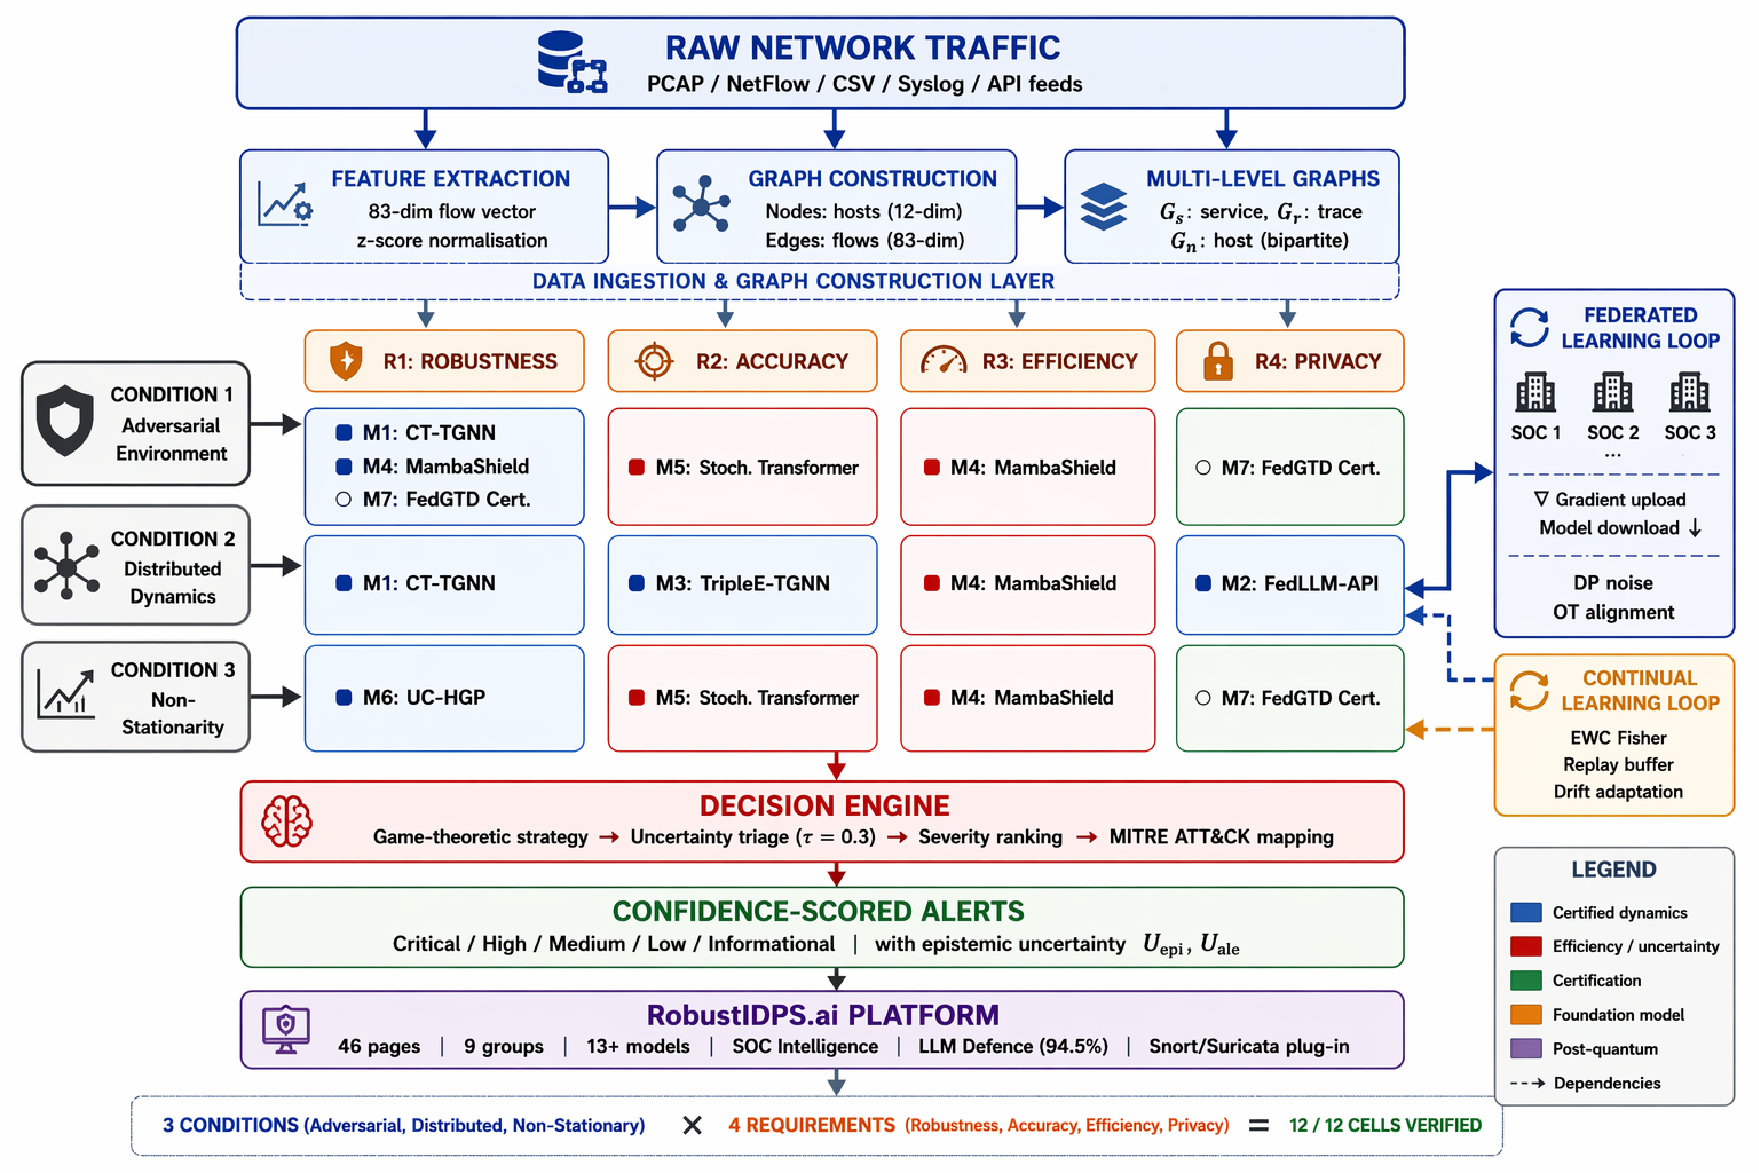
\includegraphics[width=0.85\textwidth]{figures/Main_arch_v1b.pdf}
\caption{Интегрированный конвейер обнаружения, показывающий поток данных от сырого сетевого трафика через все семь методов к оповещениям, ранжированным по серьёзности и оценённым по уверенности. Модуль FedLLM-API синхронизирует модели через границы при дифференциальной приватности.}
\label{fig:u_idps_arch}
\end{figure}

Система предназначена для развёртывания как плагин для существующих систем СОПВ, таких как Snort~3~\cite{Roesch1999} и Suricata, принимая их потоки оповещений в качестве дополнительного входа и формируя обогащённые выходы с оценкой уверенности. Полная программная реализация описана в Главе~\ref{ch:platform}, публично архивирована под DOI 10.5281/zenodo.19129512~\cite{Anaedevha2026robustidps}.
%%====

%%=====================================================================

%%=====================================================================
%%   ЭТАЛОННАЯ ВАЛИДАЦИЯ СИСТЕМЫ HYBRID IDPS НА СЕТЕВОМ ТРАФИКЕ
%%   (Перенесено из бывшей Главы~4 §§4.1-4.5 в составе Phase 2.5
%%   реорганизации Опции~Б: NIDS-инстанцирование и его эталонная
%%   валидация объединены в одну главу.)
%%====

% Связующий параграф перед методологией.
\medskip
\noindent\emph{Связь с предыдущим:} разделы~\ref{sec:nidps_context}--\ref{sec:integrated_arch}
сформировали инстанцирование гибридной СОПВ для задачи защиты
сетевого трафика на уровне сущностей, признаков, гиперпараметров и
интегрированной архитектуры. Разделы~\ref{sec:exp_methodology}--\ref{sec:ablation}
ниже систематически валидируют эту реализацию системы на шести
эталонных наборах данных, обеспечивая прямое сопоставление
результатов с инвариантами~П2--П6 из~\S\ref{subsec:six_properties}.
%%====

%%=====================================================================

%%=====================================================================
\section{Обеспечение воспроизводимости результатов и распространение программного комплекса}
\label{sec:reproducibility}

Воспроизводимость результатов диссертационного исследования обеспечивается
\emph{полным} депонированием исходного кода, обученных моделей и
экспериментальных протоколов в открытом репозитории Zenodo
(DOI:~10.5281/zenodo.19129512).

\textbf{Публикация исходного кода.} Все компоненты платформы
RobustIDPS.ai, включая 17 нейросетевых моделей, серверный ярус
(FastAPI/Python), клиентский ярус (React/TypeScript) и плагин для
Suricata EVE-JSON, опубликованы под открытой лицензией. Полный
\texttt{requirements.txt} (Python) и \texttt{package.json} (Node.js)
с зафиксированными версиями зависимостей депонированы вместе с кодом.

\textbf{Описание программных компонентов.} Каждый компонент сопровождается
техническим описанием интерфейсов, входных и выходных форматов данных,
параметров запуска и зависимостей; описания структурированы в виде
\texttt{README.md} и каталога \texttt{docs/} с разделением по
функциональным группам.

\textbf{Документация и средства воспроизведения экспериментов.}
Скрипты\,/\,Makefile-цели обеспечивают однокомандный запуск всех
ключевых экспериментов на эталонных наборах данных; конфигурации
гиперпараметров, разделения выборок и параметры оценки фиксированы в
YAML-файлах.

\textbf{Вклад в проекты с открытым исходным кодом.} Производные
наработки, имеющие самостоятельную ценность вне диссертационной работы
(плагин Suricata EVE-JSON, обёртки PyTorch\,Geometric для непрерывно
эволюционирующих графов), переданы в соответствующие upstream-проекты
в виде pull-request-ов.
%%====
\section{Выводы по разделу 3}
\label{sec:ch3_summary}
%%====

В настоящей главе систематически разработана и программно
реализована система \textbf{RobustIDPS.ai}~--- инстанциация
математической модели гибридной СОПВ из Главы~\ref{ch:methods}
для сектора защиты сетевого трафика. Глава имеет \emph{исключительно
программно-разработческий характер}: экспериментальные исследования
качества разработанной системы и её количественная валидация на
эталонных наборах данных вынесены в Главу~\ref{ch:experiments}.

Ключевые программно-инженерные вклады главы:
\begin{itemize}\setlength\itemsep{2pt}
\item \emph{(1)}~Формализован конвейер преобразования сырого
трафика форматов PCAP и CSV в темпоральные графовые структуры с
признаками узлов (12 измерений) и рёбер (83 измерения),
систематически реализующий компоненты
$(\calV_t, \calE_t, X_t, A_t)$ кортежа гибридной СОПВ
из~\eqref{eq:hybrid_idps_tuple}.
\item \emph{(2)}~Разработана унифицированная таксономия классификации
из 34~классов по 7~категориям атак, расширяемая через
zero-shot-классификацию большой языковой модели и систематически
задающая множество значений детектора~$f_\theta$.
\item \emph{(3)}~Реализован комплексный конвейер инженерии
83~признаков, охватывающий статистику потоков, распределения
межпакетных интервалов, флаговые индикаторы, статистику полезной
нагрузки и производные отношения.
\item \emph{(4)}~Выполнена NIDS-ориентированная программная
реализация всех семи моделей~М1--М7 с гиперпараметрами,
постоянными времени и архитектурными конфигурациями,
адаптированными под требования сектора защиты сетевого трафика.
\item \emph{(5)}~Разработана единая интегрированная архитектура
системы, демонстрирующая сквозной поток обработки от сырого
трафика до оповещений оператора SOC с оценкой уверенности и
автоматизированным реагированием.
\item \emph{(6)}~Реализован технологический стек промышленного
уровня (FastAPI/PyTorch~2.x с расширениями PyTorch~Geometric и
DGL, React~18 / прогрессивное веб-приложение, PostgreSQL~16,
Redis~7, Docker~Compose), включая интеграцию четырёх коммерческих
LLM-провайдеров и плагин для Suricata EVE-JSON.
\item \emph{(7)}~Разработан 51-страничный пользовательский интерфейс
прогрессивного веб-приложения, объединяющий 17~нейросетевых
моделей в 10~функциональных групп; продемонстрирован типичный
сценарий работы аналитика SOC.
\end{itemize}

Совокупность реализованных компонентов составляет программную
платформу \textbf{RobustIDPS.ai}, депонированную в репозитории Zenodo
(DOI: 10.5281/zenodo.19129512) с открытым исходным кодом.
\emph{Количественная экспериментальная валидация разработанной
системы~--- оценка качества обнаружения, состязательной
устойчивости, эффективности, приватности, калибровки,
абляционные исследования и кросс-доменный перенос~--- представлена
в Главе~\ref{ch:experiments}.}

